% Este documento destina-se a servir como modelo para a produção de documentos
% de pesquisa do PPGINF/UFPR, como projetos, dissertações e teses. A classe de
% documento se chama "ppginf" (arquivo ppginf.cls) e define o formato básico do
% documento. O texto está organizado em capítulos que são colocados em
% subdiretórios separados. São definidos exemplos para a inclusão de figuras,
% códigos-fonte e a definição de tabelas.
%
% Produzido por Carlos Maziero (maziero@inf.ufpr.br) em Outubro de 2015.
% Adaptado de um modelo anterior construído pelo autor para o PPGIA/PUCPR.

% Opções da classe ppginf:
%
% - defesa  : versão para entregar à banca; tem espaçamento 1,5
%             e omite algumas páginas iniciais (agradecimentos, etc)
% - final   : versão pós-defesa, para enviar à biblioteca;
%             tem espaçamento simples e todas as páginas iniciais.
% - oneside : para impressão somente frente; use quando for gerar
%             somente o PDF, sem impressão.
% - twoside : para impressão frente/verso; use quando for gerar
%             uma versão impressa, para economizar papel.
% - ... (demais opções aceitas pela classe "book")

% Opções default: defesa, oneside
\documentclass[defesa,oneside]{ppginf}	% versão para a defesa
%\documentclass[final,oneside]{ppginf}	% versão final, só em PDF
%\documentclass[final,twoside]{ppginf}	% versão final, em PDF + impresso

% configurações de diversos pacotes, inclusive o fonte principal do texto
% Pacotes usados neste documento e suas respectivas configurações

% ------------------------------------------------------------------------------

% seleção de línguas do texto (a última é a principal/default)
\usepackage[english,brazilian]{babel}
\selectlanguage{brazilian}

% ------------------------------------------------------------------------------
% Definição de fontes

% formato dos arquivos-fonte (utf8 no Linux e latin1 no Windows)
\usepackage[utf8]{inputenc}	% arquivos LaTeX em Unicode (UTF8)

% usar codificação T1 para ter caracteres acentuados corretos no PDF
\usepackage[T1]{fontenc}

% fonte usada no corpo do texto (descomente apenas uma)
\usepackage{newtxtext,newtxmath}	% Times (se não tiver, use mathptmx)
%\usepackage{lmodern}			% Computer Modern (fonte clássico LaTeX)
%\usepackage{kpfonts}			% Kepler/Palatino (idem, use mathpazo)
%\renewcommand{\familydefault}{\sfdefault} % Arial/Helvética (leia abaixo)

% A biblioteca central da UFPR recomenda usar Arial, seguindo a recomendação da
% ABNT. Essa é uma escolha ruim, pois fontes sans-serif são geralmente inade-
% quados para textos longos e impressos, sendo melhores para páginas Web.
% http://www.webdesignerdepot.com/2013/03/serif-vs-sans-the-final-battle/.

% fontes usadas em ambientes específicos
\usepackage[scaled=0.9]{helvet}		% Sans Serif
\usepackage{courier}			% Verbatim, Listings, etc

% ------------------------------------------------------------------------------

% inclusão de figuras
\usepackage{graphicx}			% incluir figuras em PDF, PNG, PS, EPS

% subfiguras (subfigure is deprecated, don't use it)
%\usepackage[labelformat=simple]{subcaption}
%\renewcommand\thesubfigure{(\alph{subfigure})}

% ------------------------------------------------------------------------------

% inclusão/formatação de código-fonte (programas)
\usepackage{listings}
\lstset{language=c}
\lstset{basicstyle=\ttfamily\footnotesize,commentstyle=\textit,stringstyle=\ttfamily}
\lstset{showspaces=false,showtabs=false,showstringspaces=false}
\lstset{numbers=left,stepnumber=1,numberstyle=\tiny}
\lstset{columns=flexible,mathescape=true}
\lstset{frame=single}
\lstset{inputencoding=utf8,extendedchars=true}
\lstset{literate={á}{{\'a}}1  {ã}{{\~a}}1 {à}{{\`a}}1 {â}{{\^a}}1
                 {Á}{{\'A}}1  {Ã}{{\~A}}1 {À}{{\`A}}1 {Â}{{\^A}}1
                 {é}{{\'e}}1  {ê}{{\^e}}1 {É}{{\'E}}1  {Ê}{{\^E}}1
                 {í}{{\'\i}}1 {Í}{{\'I}}1
                 {ó}{{\'o}}1  {õ}{{\~o}}1 {ô}{{\^o}}1
                 {Ó}{{\'O}}1  {Õ}{{\~O}}1 {Ô}{{\^O}}1
                 {ú}{{\'u}}1  {Ú}{{\'U}}1
                 {ç}{{\c{c}}}1 {Ç}{{\c{C}}}1 }

% ------------------------------------------------------------------------------

% formatação de algoritmos
\usepackage{algorithm,algorithmic}
\floatname{algorithm}{Algoritmo}
\renewcommand{\algorithmiccomment}[1]{~~~// #1}
%\algsetup{linenosize=\footnotesize,linenodelimiter=.}

% ------------------------------------------------------------------------------

% listas de símbolos e de abreviações (a fazer)
%\usepackage[titles]{tocloft}
%\newlistof[part]{symb}{los}{Lista de Símbolos}
%\newlistof[part]{abbrev}{loa}{Lista de Abreviações}
%\newcommand{\symb}[2]{%
%\refstepcounter{symb}
%\addcontentsline{los}{symb}{\protect #1 :#2}\par}

% ------------------------------------------------------------------------------

% formatação de bibliografia
\usepackage{natbib}		% bibliografia no estilo NatBib

% ------------------------------------------------------------------------------

% outros pacotes diversos
\usepackage{alltt,moreverb}	% mais comandos no modo verbatim
\usepackage{lipsum}		% gera texto aleatório (para os exemplos)
\usepackage{currfile}		% infos sobre o arquivo/diretório atual
\usepackage[final]{pdfpages}	% inclusão de páginas em PDF
\usepackage{longtable}		% tabelas multi-páginas (tab símbolos/acrônimos)

% ------------------------------------------------------------------------------



%=====================================================

\begin {document}

% Principais dados, usados para gerar as páginas iniciais.
% Campos não utilizados podem ser removidos ou comentados.

% título :-)
\title{Modelo conceitual para mitigar a propagação de informações falsas em redes sociais }

% palavras-chave e keywords
\pchave{credibilidade, informação, notícias falsas, autoridade cognitiva, rede social, avaliação de credibilidade, qualidade de informação, classificação de informação}
\keyword{information, credibility, fake news, cognitive authority, social network, evaluation of credibility, information quality, information classification}

% autoria
\author{Lucas Nathan Barbosa de Oliveira}
\advisor{Roberto Pereira}
%\coadvisor{Leslie Lamport}
\instit{UFPR}{Universidade Federal do Paraná}

% área de concentração (default do PPGInf, não mudar)
\field{Ciência da Computação}

% local e data
\date{2018}
\local{Curitiba PR}

% imagem de fundo da capa (comentar se não desejar)
\coverimage{0-iniciais/fundo-capa.jpg}

%% Descrição do documento (obviamente, descomentar somente UMA!)

% tese de doutorado
%\descr{Tese apresentada como requisito parcial à obtenção do grau de Doutor em Informática, no Programa de Pós-Graduação em Informática, setor de Ciências Exatas, da Universidade Federal do Paraná}

% exame de qualificação de doutorado
%\descr{Documento apresentado como requisito parcial para o exame de qualificação de Doutorado, no Programa de Pós-Graduação em Informática, setor de Ciências Exatas, da Universidade Federal do Paraná}

% dissertação de mestrado
%\descr{Dissertação apresentada como requisito parcial à obtenção do grau de Mestre em Informática, no Programa de Pós-Graduação em Informática, setor de Ciências Exatas, da Universidade Federal do Paraná}

% exame de qualificação de mestrado
\descr{Documento apresentado como requisito parcial para o exame de qualificação de Mestrado, no Programa de Pós-Graduação em Informática, setor de Ciências Exatas, da Universidade Federal do Paraná}

% trabalho de conclusão de curso
%\descr{Trabalho apresentado como requisito parcial à conclusão do Curso de Bacharelado em XYZ, setor de Ciências Exatas, da Universidade Federal do Paraná}

% trabalho de disciplina
%\descr{Trabalho apresentado como requisito parcial à conclusão da disciplina XYZ no Curso de Bacharelado em XYZ, setor de Ciências Exatas, da Universidade Federal do Paraná}

%=====================================================

% define estilo das páginas iniciais (capas, resumo, sumário, etc)
\frontmatter
\pagestyle{frontmatter}

% define capa e folha de rosto
\titlepage

% páginas que só aparecem na versão final (a inclusão é automática)
%% - IMPORTANTE - IMPORTANTE - IMPORTANTE - IMPORTANTE -
%
% O conteúdo exato da ficha catalográfica é preparada pela Biblioteca Central
% da UFPR, a pedido da secretaria do PPGINF. Não "invente" um conteúdo para ela,
% se informe a respeito com a secretaria do programa.

\begin{ficha}	% só gera conteúdo se for na versão final

% inclusão da ficha catalográfica final (arquivo PDF)
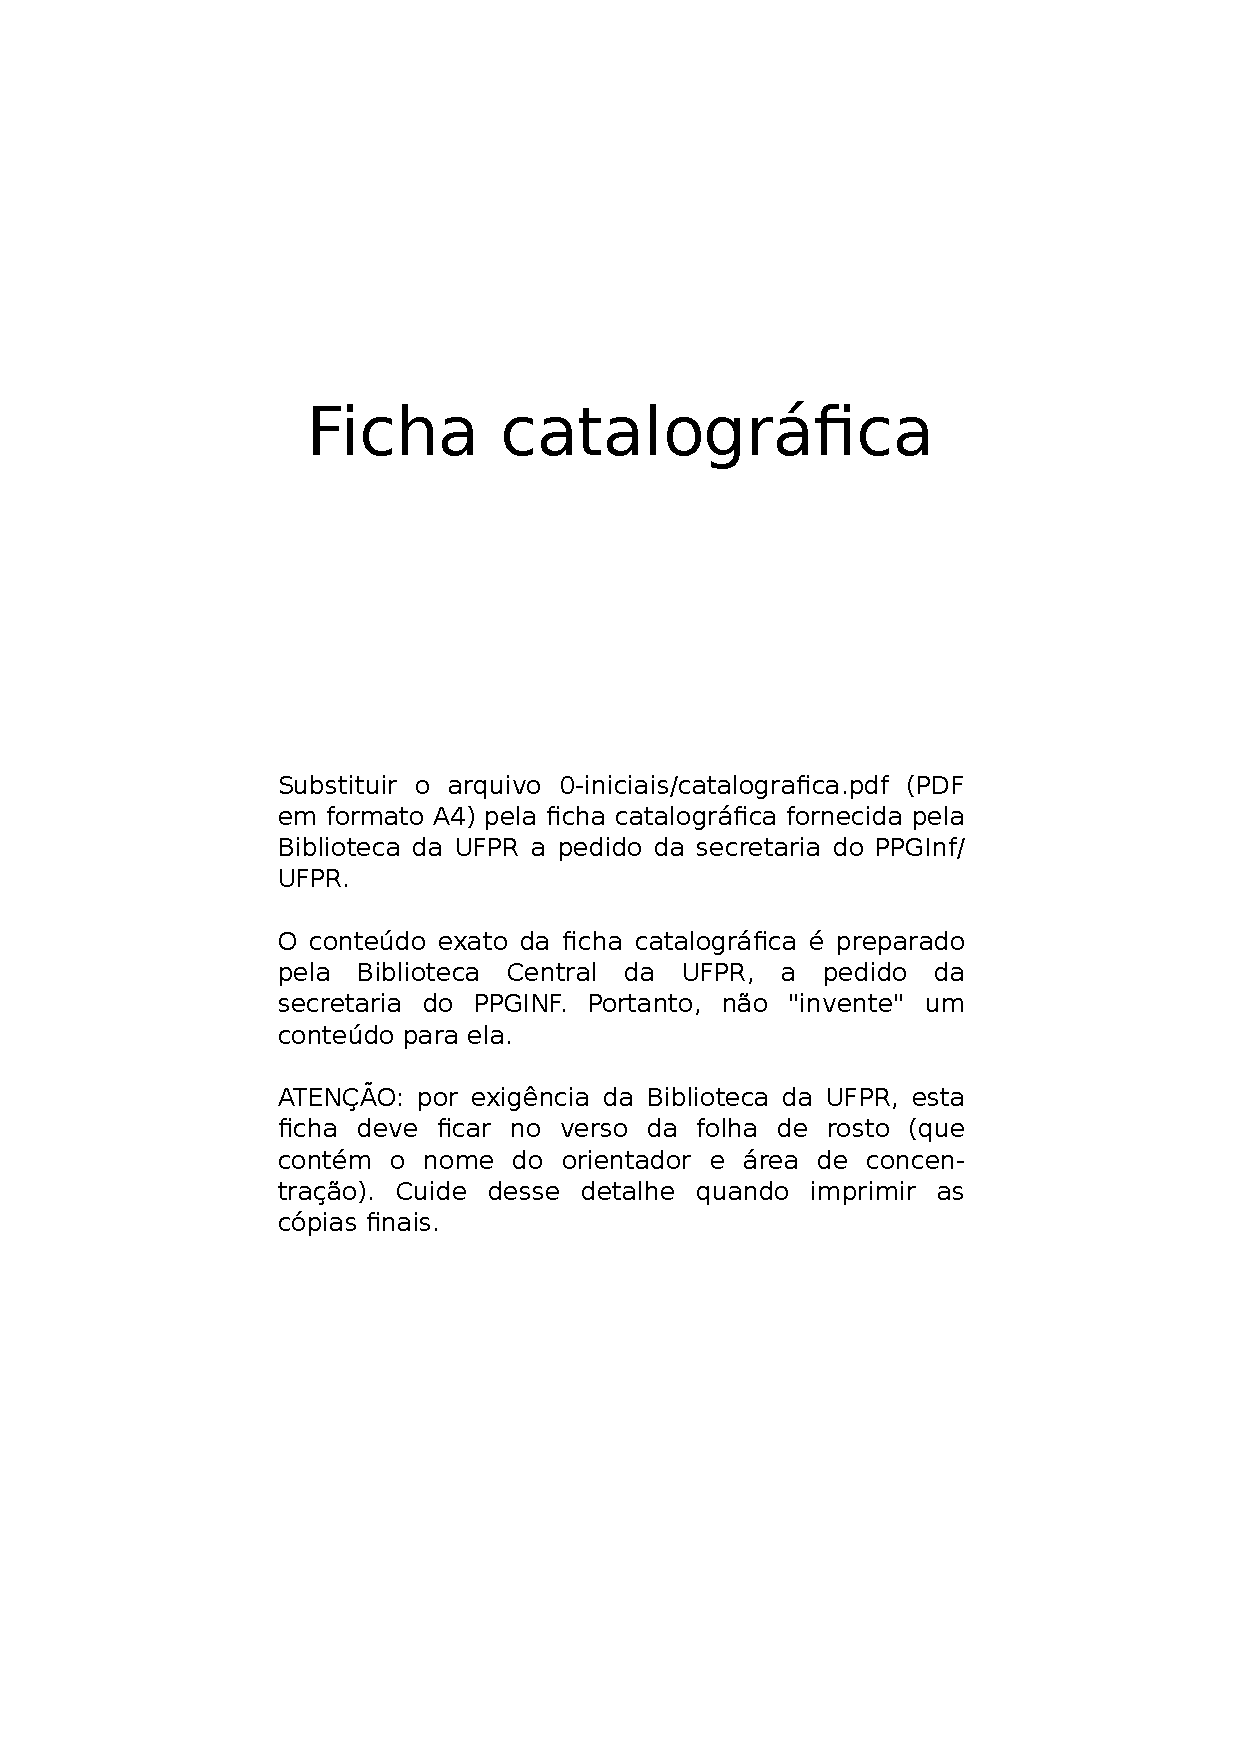
\includepdf[noautoscale]{0-iniciais/catalografica.pdf}

\end{ficha}

%=====================================================
	% ficha catalográfica
%% A ficha de aprovação será fornecida pela secretaria do programa,
% após a defesa e cumprimento dos demais trâmites legais.

\begin{aprovacao}	% só gera conteúdo se for na versão final

% inclusão do termo de aprovação final (arquivo PDF)
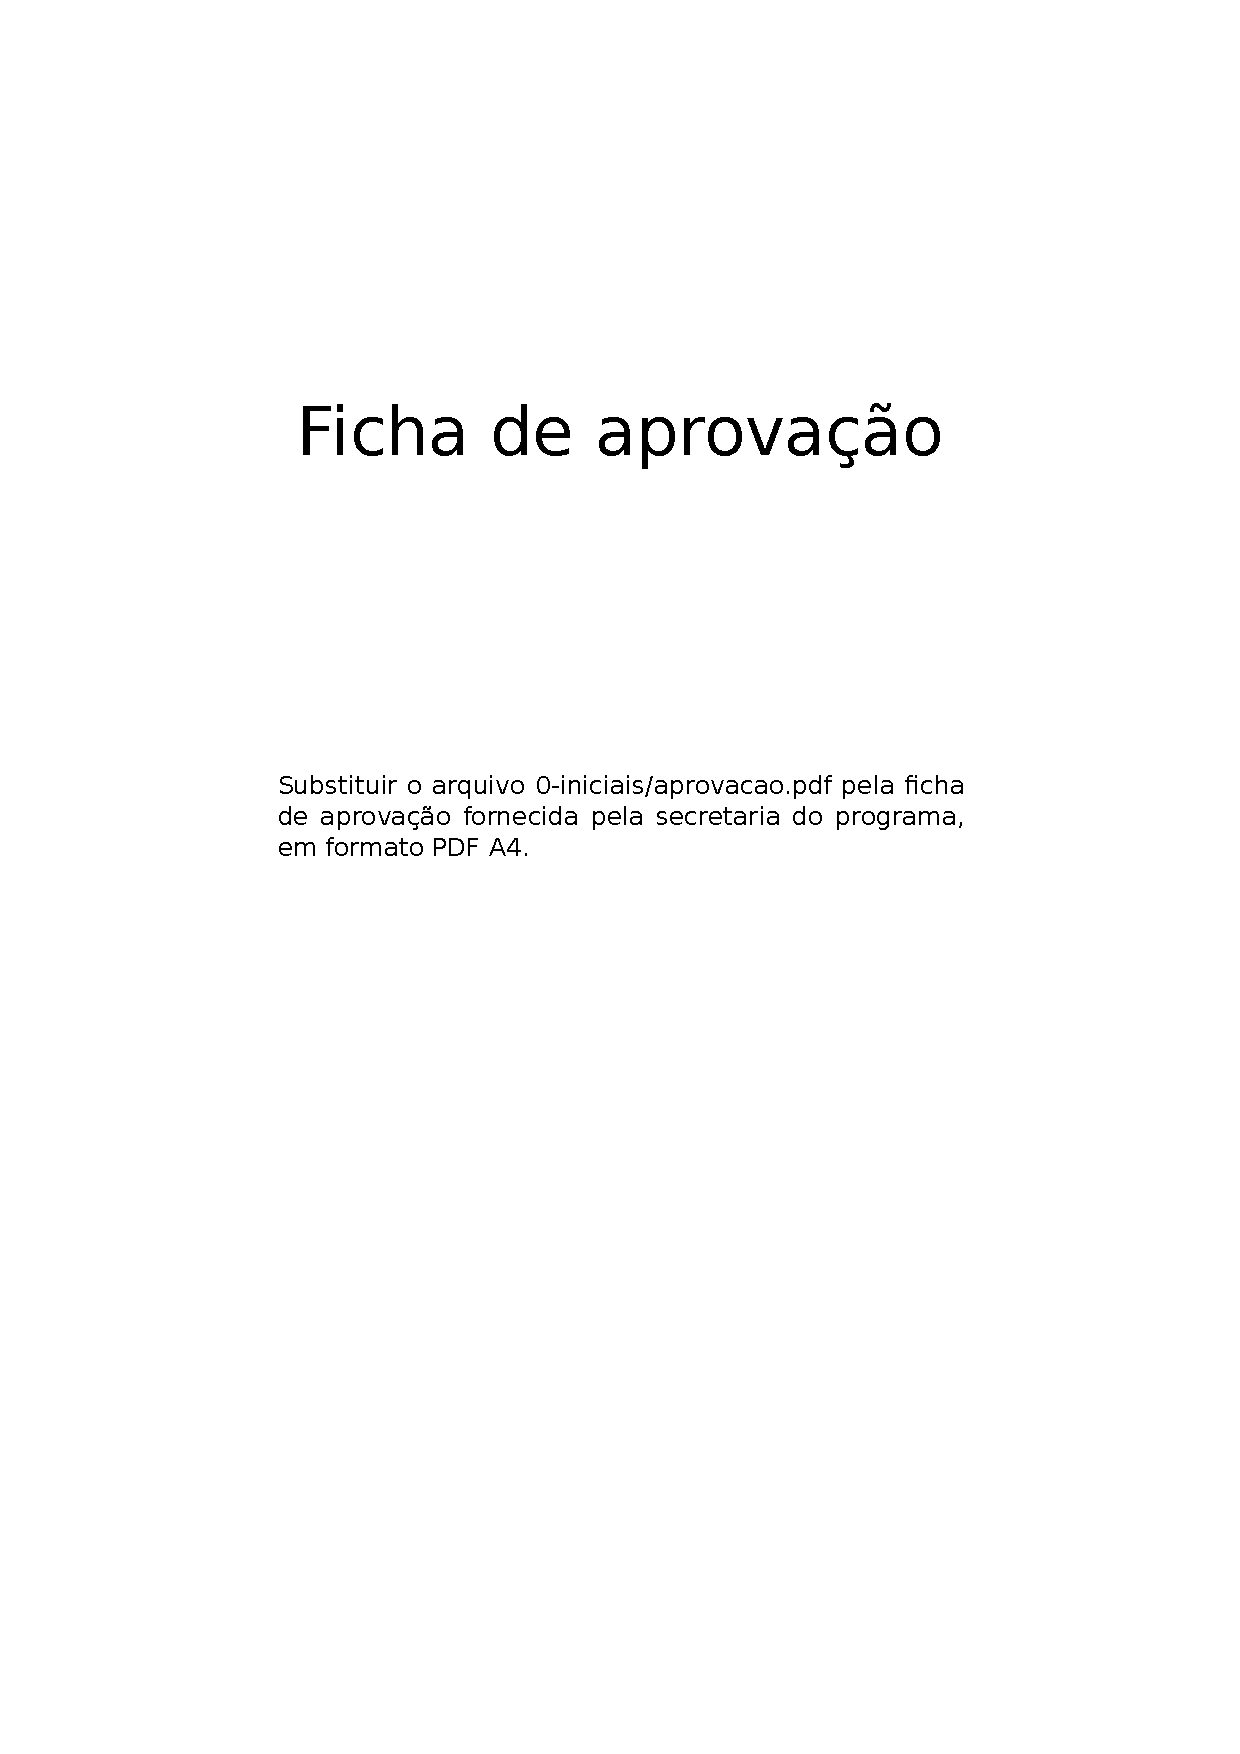
\includepdf[noautoscale]{0-iniciais/aprovacao.pdf}

\end{aprovacao}

%=====================================================
		% folha de aprovação
%\begin{dedica}  % só gera conteúdo se for na versão final

A alguém...

\end{dedica}

		% dedicatória
%\begin{agradece}	% só gera conteúdo se for na versão final

Inserir os agradecimentos. Os agradecimentos devem ocupar no máximo uma página, devem ser justificados na largura da página e com um afastamento de parágrafo na primeira linha de 1,27 cm. O espaçamento entre linhas deve ser de 1,5 linhas. Não deve haver espaçamento adicional entre parágrafos.

\lipsum[2-5]	% gera um texto aleatório

\end{agradece}

		% agradecimentos

% resumo (português) e abstract (inglês), nesta ordem
\begin{resumo}

As redes sociais facilitaram o compartilhamento de informações entre as pessoas, fornecendo um ambiente com baixo ou nenhum filtro de publicação, onde o conteúdo criado por uma pessoa pode alcançar milhões, resultando em uma sobrecarga de informação, que pode confundir e/ou enganar os usuários da rede. Além disso, as pessoas estão cada vez mais utilizando estes ambientes para acessar notícias que outrora procuravam em noticiários especializadas. Portanto, quanto maior a influência exercida por essas plataformas sob as pessoas, maior a necessidade de avaliar seus conteúdos e diferenciar as informações falsas e enganosas das verdadeiras e informativas. Para que isso seja possível este trabalho propõe a utilização de um conceito fundamentado da epistemologia social, que descreve o modo como as pessoas identificam, reconhecem e atribuem autoridade umas às outras, conhecido como teoria da autoridade cognitiva. A hipótese considerada é de que os fundamentos da teoria da autoridade cognitiva podem auxiliar na classificação de notícias e na identificação de informação falsa em redes sociais. Propõe-se então, um modelo conceitual a ser implementado na forma de um protótipo de software, que considera uma avaliação de maneira quantitativa, através do desenvolvimento de cenários que irão exemplificar situações onde ocorrem a necessidade de classificar uma informação e identificar a sua qualidade. Estes cenários irão fornecer o conjunto de dados que será utilizado para validar ou refutar a hipótese.

\end{resumo}


\begin{otherlanguage}{english}

\begin{abstract}

% em inglês, o primeiro parágrafo não deve ser indentado
\noindent

Social networks have facilitated the sharing of information between people by providing an environment with low or no publishing barriers, where content created by a person can reach millions resulting in an overload of information that can confuse and/or mislead the user. In addition, people are increasingly using these environments to access news they once sought in specialized news institutions. Therefore, the greater the influence exerted by these platforms, the greater is the need to evaluate their content and to differentiate false and misleading information from truthful and informative ones. For this to be possible this paper proposes the use of a well-founded concept of social epistemology, which describes how people identify, recognize, and attribute authority to one another, known as the theory of cognitive authority. The hypothesis considered is that the foundations of the theory of cognitive authority can aid in the classification of news and the identification of false information in social networks. It is proposed a conceptual model to be implemented in the form of a software prototype, which considers an evaluation in a quantitative way, through the development of scenarios that will exemplify situations where the need to classify information and identify its quality occur. These scenarios will provide the dataset that will be used to validate or refute the hypothesis.

\end{abstract}

\end{otherlanguage}



% define sumário e demais listas (figuras, tabelas, abreviações/siglas, símbolos)
\tableofcontents
\listoffigures
\listoftables
%=====================================================

% lista de acrônimos (siglas e abreviações)

\begin{listaacron}

\begin{longtable}{p{0.2\linewidth}p{0.7\linewidth}}
DINF & Departamento de Informática\\
PPGINF & Programa de Pós-Graduação em Informática\\
UFPR & Universidade Federal do Paraná\\
FN & \emph{Fake News}\\
AC & Autoridade Cognitiva\\
RS & Redes Sociais \\
URL & \emph{Uniform Resource Locator} \\
API & \emph{Application Programming Interface} \\
\end{longtable}

\end{listaacron}

%=====================================================
		% ainda deve ser preenchida à mão
%%=====================================================

% lista de símbolos

\begin{listasimb}

\begin{longtable}{p{0.2\linewidth}p{0.7\linewidth}}
$\alpha$ & alfa, primeira letra do alfabeto grego\\
$\beta$ & beta, segunda letra do alfabeto grego\\
$\gamma$ & gama, terceira letra do alfabeto grego\\
$\omega$ & ômega, última letra do alfabeto grego\\
$\pi$ & pi \\
$\tau$ & Tempo de resposta do sistema\\
$\theta$ & Ângulo de incidência do raio luminoso\\
\end{longtable}

\end{listasimb}

%=====================================================
		% idem

%=====================================================

% define estilo do corpo do documento (capítulos e apêndices)
\mainmatter
\pagestyle{mainmatter}

% inclusao de cada capítulo, alterar a gosto (do professor de Metodologia)
\setcounter{page}{1}
%=====================================================

% A introdução geral do documento pode ser apresentada através das seguintes seções: Desafio, Motivação, Proposta, Contribuição e Organização do documento (especificando o que será tratado em cada um dos capítulos). O Capítulo 1 não contém subseções\footnote{Ver o Capítulo \ref{cap-exemplos} para comentários e exemplos de subseções.}.

\chapter{Introdução}

%tentei colocar a justificativa, e os objetivos aqui... pode ser assim?

\section{Motivação e contextualização}

Redes sociais (como \emph{Facebook, Google+, Twitter, etc...}) são populares mundialmente, permitindo que usuários conversem uns com os outros, organizem eventos, compartilhem opiniões, fotografias, artigos, informações e ainda permitem que eles construam conexões entre si. De acordo com \cite{boyd_social_2007}, um site de rede social é um serviço online que permite que indivíduos: (1) construam um perfil público ou semi-publico dentro do sistema; (2) articulem uma lista de outros usuários que compartilham uma conexão; e (3) visualizem e cruzem sua lista de contatos com as listas feitas por outros usuários. Ainda segundo \cite{boyd_social_2007} essas plataformas são bastante variadas nos seus propósitos e culturas, enquanto algumas são direcionadas à um público diversificado, outras são focados em atrair pessoas que compartilham características comuns. Na maior parte dos casos esses sites conectam pessoas que possuem vínculos fora do ambiente online, e estendem essas conexões permitindo que os usuários se articulem na rede através da troca de informações e da expansão de suas próprias redes de contato.

Existe uma facilidade de comunicação entre pessoas que participam dessas redes. No entanto quanto maior o número de usuários maior a sobrecarga de informações, o que pode confundir os usuários e fornecer o ambiente perfeito para a proliferação de conteúdos falsos e informações não verificáveis. A pesquisa realizada por \cite{nic_newman_digital_2017} do Instituto Reuters confirma este pensamento, mostrando que nos últimos seis anos houve um grande crescimento no número de pessoas que utilizam redes sociais online para acessar notícias diárias. Nos Estados Unidos mais da metade das amostras (51\%) acessam suas notícias através das mídias sociais, 5\% a mais que no ano de 2016 e o dobro em relação ao ano de 2013. Além disso, os resultados indicam que no Brasil o uso de aplicativos de mensagens (\emph{Facebook Messenger, WhatsApp e Telegram}) como fonte de informação tem crescido a ponto de rivalizar com os sites de redes sociais. A pesquisa conclui que o crescimento dos aplicativos de mensagem devem-se a privacidade fornecida pelos mesmos e a falta de filtro nas informações compartilhadas.

Segundo \cite{rasmus_kleis_nielsen_news_2017} o grande fluxo de desinformação em torno da eleição presidencial de 2016 alarmou o mundo para o problema das notícias falsas (popularizado pelo termo em inglês, \emph{Fake News}) que circulavam nas redes sociais, este termo têm ganho uma grande importância desde então. Consequentemente, a avaliação da credibilidade das informações que circulam nesses ambientes têm se transformado em um tópico de extrema importância.

% da pra colocar alguns casos de fake news aqui para dar mais forca ao argumento....

\cite{allcott_social_2017} definem \emph{fake news} como sendo artigos de notícia intencionalmente falsos, que podem ser verificados como falsos, e que podem enganar leitores. Entretanto existem outros colegas de \emph{fake news} que são deixados de fora desta definição: (1) erros cometidos por acidente; (2) rumores que não se originaram de um artigo em particular; (3) teorias da conspiração (essas são por natureza difíceis de verificar como verdadeiras ou falsas); (4) sátiras que dificilmente seriam confundidas como verdade; (5) falsas declarações de políticas; (6) relatórios que são tendenciosos mas não completamente falsos.


% discutir sobre alguns casos historicos de fake news fora do ambiente online

Porém a disseminação de notícias falsas, boatos, desinformação e fraudes não são algo novo. \cite{robert_darnton_true_2017} cita que em 1522 Pietro Aretino tentou manipular a eleição pontifícia, escrevendo sonetos perversos sobre todos os candidatos (exceto o favorito de seus patronos, os Medici) e colando-os no busto de uma figura conhecida como Pasquino para que o público os vissem, perto da \emph{Piazza Navona} em Roma . O \emph{"pasquinate"} (em italiano), em seguida, tornou-se um gênero comum de difundir notícias desagradáveis, a maioria falsa, sobre figuras públicas.

Embora as pasquinagens (em português) nunca tenham desaparecido, foram sucedidos no século XVII por um gênero mais popular, o \emph{"canard"}, uma versão da notícia falsa que se alastrou pelas ruas de Paris nos próximos duzentos anos. Os \emph{canards} eram impressos às vezes com design e gravuras para parecerem mais crédulos. Um \emph{best-seller} da década de 1780 anunciou a captura de um monstro no Chile que deveria ser enviado para a Espanha. Tinha a cabeça de uma Fúria, asas como um morcego, um corpo gigantesco coberto de escamas e uma cauda semelhante a de um dragão. Durante a Revolução Francesa, os gravadores inseriram o rosto de Marie-Antoinette nas antigas placas de cobre, e o \emph{canard} assumiu uma nova vida, desta vez como propaganda política intencionalmente falsa. Embora seu impacto não possa ser medido, certamente contribuiu para o ódio patológico da rainha, o que levou à sua execução em 16 de outubro de 1793.

Portanto, pode-se perceber que redes sociais online não contribuíram para a criação do fenômeno da disseminação das notícias falsas. Entretanto, proporcionou um ambiente propício para que essas informações se alastrassem de forma viral. 

\section{Objetivo}

O objetivo deste trabalho é fornecer artifícios que auxiliem os brasileiros a decidir em quais informações confiar nos ambientes de redes sociais. E a hipótese levantada é que a aplicação conceitos de Autoridade Cognitiva em redes sociais auxilia na identificação de notícias falsas e das entidades que as produzem. 

\section{Estrutura da proposta}

Para alcançar este objetivo destaca-se a necessidade de desenvolvimento de todas as etapas da proposta pois nenhum processo, que visa a solução de um problema, pode ser considerado completo até que uma avaliação deste seja realizada (\cite{jayaratna_understanding_1994}).

\begin{itemize}
    \item \textbf{Modelo conceitual:} Este será um modelo de rede social fundamentado na teoria de Autoridade Cognitiva (AC) de \cite{Wilson1983}, explorando a natureza colaborativa e informal da Internet;
    \item \textbf{Protótipo:} O protótipo irá por em prática as ideias apresentadas no modelo citado, é a partir desta implementação que o modelo será avaliado;
    \item \textbf{Experimentos e avaliação:} O experimento irá por a prova o modelo e a implementação do protótipo a fim de validar a hipótese apresentada. Serão então desenvolvidos cenários que desafiarão a hipótese, afim de descobrir se ela é válida, inválida ou se é válida em cenários específicos.
\end{itemize}



%essa definição foi a que eu achei mais interessante, mas ainda fico em dúvida sobre utilizar a 5 e a 6



%mostra que Devemos também ponderar o motivo das pessoas não confiarem nos meios de comunicação atuais. Segundo a pesquisa realizada por \cite{nic_newman_bias_2017}, as matérias imparciais, tendenciosas e com motivos próprios (além do repasse de informação) por parte das agências de jornalismo são as maiores razões para as pessoas perderem a confiança nos meios de comunicação, piorado pelo declínio dos padrões de publicação, acarretados pela competição com os novos modelos de negócio online. Para concluir, o estudo diz que a confiança que as pessoas depositam nos conteúdos vistos nas redes sociais é baixo, porém aponta que isso acontece em função do modelo em prática, que permite que qualquer um publique sem checagem de fatos, ou com com algoritmos que as vezes favorecem conteúdos extremos ou controversos.

%\section{Objetivos}

%A proliferação de notícias falsas, boatos e desinformação não é um problema novo na nossa sociedade, segundo \cite{pfaltzgraff_soviet_1981}, no decorrer da história da humanidade a desinformação foi utilizada como meio de controle de massas e de desestabilização de nações antes da popularização da Internet. Portanto, a popularização das redes sociais apenas forneceram artifícios que contribuíram para o aumento do problema. 			% introdução
\chapter{Fundamentação Teórica}

% fundamentação teórica
%---------------------------------------------------------------------------------------------------------------------
\section{Redes Sociais}

Redes sociais online têm atraído milhões de usuários que integraram essas plataformas nos seus dia-a-dia. Essas plataformas são bastante variadas nos seus propósitos e culturas, enquanto algumas são direcionadas a um publico diversificado, outros são focados em atrair pessoas que compartilham características comuns. De acordo com \cite{boyd_social_2007} um site de rede social é um serviço online que permite que seus usuários:

\begin{enumerate}
    
    \item \textbf{Construam um perfil público ou semi-publico dentro do sistema}: Este perfil é gerado utilizando uma série de formulários que podem conter algumas questões pessoais sobre o participante como idade, nome, localidade, interesses ou profissão. Alguns sites permitem que usuários personalizem seus perfis permitindo a adição de mídias como fotos e vídeos, ou modifiquem a interface da página de perfil;
    
    \item \textbf{Articulem uma lista de outros usuários que compartilham uma conexão}: Após se juntar a uma rede social, os usuários podem identificar outras pessoas no sistema, que eles possuam uma conexão. Esse relacionamento pode variar em nomenclatura dependendo do site, os termos "Amigos" e "Contatos" estão entre os mais comuns. O relacionamento pode ser de duas maneiras: \textbf{(1) bidirecional}, onde a conexão só é formada com a confirmação de "amizade" entre os dois usuários da rede, ou \textbf{(2) unidirecional}, indicando que uma pessoa pode possuir a outra na lista de contato, mas a recíproca pode não ser verdadeira, como o recurso de ``seguir'' utilizado pela plataforma \emph{Twitter};
    
    \item \textbf{Organizem e cruzem sua lista de contatos com as listas feitas por outros usuários}: Isso pode ser alcançado de várias maneiras, entre elas: (1) a lista de contatos do usuário possui um link direcionando para a lista de contatos de cada usuário em sua rede, permitindo a visualização e a interação com diferentes redes sociais, (2) o próprio site propõe usuários com interesses semelhantes, através de um algoritmo que cruza informações obtidas através de seus perfis. Geralmente são utilizadas uma dessas estratégias, as duas, ou mistura delas.
    
\end{enumerate}

\cite{boyd_social_2007} apontam que os sites de redes sociais geralmente fornecem um mecanismo para que os usuários deixem mensagens uns para os outros de forma pública ou privada. Além disso, alguns sites fornecem varias outras funcionalidades como: compartilhamento de fotos, vídeos, mensagens, artigos, \emph{urls}, escrita de blog, etc. Variando de acordo com o objetivo principal de cada site.

Segundo \cite{haythornthwaite_social_2005} o que faz esses sites tão interessantes para o público é sua capacidade de permitir que os usuários interajam com as redes sociais uns dos outros. Isso pode resultar em conexões entre pessoas, que não aconteceriam de outra maneira. Porém este não é o objetivo, e essas conexões frequentemente acontecem entre pessoas que possuem um "laço latente", uma conexão offline. \cite{boyd_social_2007} discutem que em muitas das grandes redes sociais os participantes não necessariamente procuram novas conexões, o principal objetivo deles é se comunicar com pessoas que já fazem parte de sua rede social. Porém, para enfatizar a característica de organização e articulação destes serviços, eles são chamados de "Sites de Redes Sociais".


%---------------------------------------------------------------------------------------------------------------------
\section{Fake News}

\cite{robert_darnton_true_2017} mostra que o termo \emph{Fake News}(FN) não é novo, e aponta que fenômenos de desinformação em massa existem a séculos e com muitos exemplos no decorrer história da humanidade. As definições encontradas na literatura são variadas, o dicionário de Cambridge\footnote{https://dictionary.cambridge.org/dictionary/english/fake-news. Acessado em 24 de Janeiro, 2018} define \emph{Fake News} como: 

\begin{quote}
    "False stories that appear to be news, spread on the internet or using other media, usually created to influence political views or as a joke"
    \footnote{Tradução do autor: "Histórias falsas que parecem ser notícias, disseminadas pela Internet ou em outro smeios de comunicação, normalmente criadas para influenciar visões políticas ou com caráter humorístico"}
\end{quote}

Já \cite{allcott_social_2017} afirmam que FN são:
\begin{quote}
    "News articles that are intentionally and verifiably false, and could mislead readers"
    \footnote{Tradução do autor: "Notícias intencionalmente falsas, podem ser verificadas como falsas, porém tem poder de enganar as pessoas que estão lendo"}
\end{quote}

A definição de \cite{allcott_social_2017} exclui alguns termos que tem sido relacionados a Fake News: (1) erros cometidos por acidente; (2) rumores que não se originaram de um artigo em particular; (3) teorias da conspiração (essas são por natureza difíceis de verificar como verdadeiras ou falsas); (4) Sátiras que dificilmente seriam confundidas como verdade; (5) falsas declarações de políticos; (6) relatórios que são tendenciosos mas não completamente falsos. Entretanto \cite{tandoc_defining_2017} discutem um termo mais abrangente e propõem um \emph{framework} baseado em definições do termo utilizadas em artigos científicos publicados entre 2003 e 2017, que é utilizado para construir uma tipologia de FN. Para entender como funciona o \emph{framework} precisamos apresentar primeiramente as seis maneiras de operacionalização de \emph{fake news} encontradas pela pesquisa de \cite{tandoc_defining_2017}:

\begin{enumerate}
    \item \textbf{Sátiras de notícias:} Utiliza-se de humor ou exagero para apresentar o conteúdo á audiência. Entretanto, o humor utilizado nessas notícias é apenas um artifício para entreter o público, e não visa descaracterização na veracidade da informação apresentada;
    
    \item \textbf{Paródias de notícias:} Muito semelhante as sátiras, as paródias também utilizam-se de humor para transmitir conteúdo. Porém, nas paródias é normal que a informação seja retorcida e que dados inventados sejam inseridos pelo bem do humor; 
    
    \item \textbf{Fabricação de notícias:} São artigos sem embasamento em fatos que se mascaram como notícias reais, tentam transmitir legitimidade e buscam ludibriar o público. A diferença entre a fabricação e a paródia de notícias está no entendimento existente entre o público e o autor.  Na paródia, o público sabe que está lendo uma notícia falsa e de caráter humorístico, na fabricação o autor busca confundir o leitor, que fica com dificuldade para decernir a veracidade do conteúdo apresentado.
    
    \item \textbf{Manipulação de multimídia:} Enquanto as outras categorias se referem a conteúdos textuais, nessa é descrita a manipulação gráfica de imagens e vídeos;
    
    \item \textbf{Publicidade e relações públicas:} Nesta categoria materiais publicitários sob a aparência de notícias genuínas. Isso acontece quando profissionais de relações públicas adotam práticas e/ou aparência de jornalistas para inserir mensagens persuasivas nos meios de comunicação. As famosas manchetes \emph{clickbait}\footnote{"Articles, photographs, etc. on the internet that are intended to attract attention and encourage people to click on links to particular websites". https://dictionary.cambridge.org/us/dictionary/english/clickbait. Acessado em 24 de Janeiro, 2018}\footnote{Tradução do autor:"Artigos, fotos, etc. na Internet que possuem a intenção de atrair atenção e encorajar as pessoas a clicar em um link em websites particulares} que utilizam o formato de noticias convencionais, mas direcionam o público para um conteúdo comercial são exemplos de FN dessa categoria;
    
    \item \textbf{Notícias tendenciosas ou propagandas políticas:} Notícias que são criadas por entidades políticas para influenciar a opinião pública. O propósito dessas notícias é beneficiar uma organização, figura pública ou governo. Similares aos anúncios publicitários, porém as propagandas geralmente são uma mistura de fatos com uma narrativa tendenciosa. São alguns exemplos de propaganda: Matérias tendenciosas e artigos com conteúdo persuasivo e unilateral.
\end{enumerate}

Analisando as categorias apresentadas nota-se que todas tentam parecer notícias legitimas, se apossando de formatos e visuais consagrados por mídias convencionais e se aproveitando da credibilidade que essas possuem. Para mapear os tipos de \emph{Fake News} \cite{tandoc_defining_2017} ainda propõe a utilização de dois domínios: \textbf{(1) facticidade}, se referindo ao grau em que a notícia se baseia em fatos reais, e \textbf{(2) intenção imediata do autor}, uma referência ao propósito do autor com a notícia, se o autor planeja enganar o público com a sua notícia ou não.

A figura \ref{fig:topologia_fn} mostra a formação de um plano cartesiano utilizando os dois domínios mencionados, este plano pode ser utilizado para mapear as diferentes categorias de FN.

\begin{figure}[!htb]
\centering
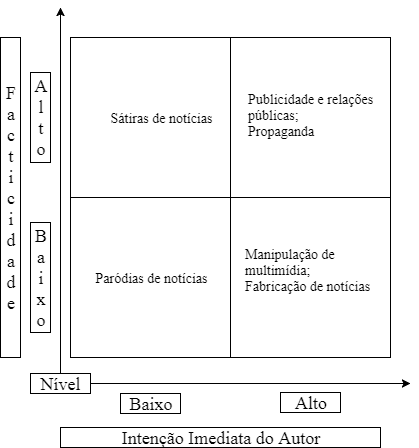
\includegraphics[width=10cm]{2-fundamentacao/typology_fake_news.png}
\caption{Tipologia de \emph{Fake News}.}
\label{fig:topologia_fn}
\end{figure}

Conclui-se então que apesar de ser muito utilizado na mídia (\cite{liliana_bounegru_field}, o termo"\emph{Fake News}" é muito abrangente e possui diferentes definições dependendo do estudo e do contexto, mas é possível mapear essas definições que podem ser utilizadas como base no nosso trabalho.

%---------------------------------------------------------------------------------------------------------------------
\section{Autoridade Cognitiva}

Em seu livro, \emph{Second-hand Knowledge: An Inquiry into Cognitive Authority} \cite{Wilson1983} apresenta a teoria da Autoridade Cognitiva (AC), desenvolvida através de um estudo da natureza social humana. Em seu trabalho ele afirma que o ser humano constrói conhecimento de duas maneiras: 
\begin{enumerate}
    \item \textbf{Primeira mão}: onde a pessoa constrói conhecimento através das suas próprias experiências;
    \item \textbf{Segunda mão}: onde a pessoa constrói conhecimento através das experiências de outras pessoas. Sendo que ele fundamenta sua teoria da Autoridade Cognitiva nesta maneira de adquirir conhecimento. 
\end{enumerate}

Wilson acredita que tudo que as pessoas conhecem do mundo fora do curto alcance das suas vidas, é o que outras pessoas contam. Ele afirma que tudo é boato, mas que nem todos os boatos são iguais, existem alguns confiáveis, aqueles que "sabem o que estão falando", e apenas esses contam como autoridades cognitivas. Ele usa o termo autoridade cognitiva para descrever alguém que influencia, que as pessoas consideram apropriado. É diferente de uma autoridade administrativa provinda de uma posição hierárquica imposta ou concedida. Portanto uma AC é alguém cujas capacidades e competências foram reconhecidas por outro indivíduo.

Wilson discute que existem vários elementos que são levados em consideração quando definimos Autoridades Cognitivas:

\begin{enumerate}
    \item \textbf{Envolve um relacionamento entre no mínimo dois atores}: uma pessoa precisa ser reconhecida por outra para ser uma autoridade cognitiva, ou reconhecer outra para que esta seja uma AC;
    
    \item \textbf{Existe um nível de AC}: uma pessoa pode ter um nível alto ou baixo de autoridade;
    
    \item \textbf{É relativo à uma área de interesse}: uma pessoa pode ter um nível alto de AC em determinado assunto, mas não ter em outro que escapa da sua linha de conhecimento;
    
    \item \textbf{AC é relacionada à credibilidade}: pois só concedemos autoridade à quem julgamos dignos de confiança, uma fonte de informação que não é considerada digna será então naturalmente descartada.
\end{enumerate}

Se uma pessoa utilizar como base de conhecimento apenas aquilo que ela vivencia, essa pessoa passa a ter ideias muito limitada, pois esse individuo tem uma período de vida curto onde não é possível experimentar tudo. É utilizando os conhecimentos de segunda mão aprendidos através da experiência de outros que uma pessoa pode expandir sua visão de mundo. Entretanto, é importante destacar que Wilson não diz que conhecimento de segunda-mão é mais importante do que vivenciar experiências diretamente (primeira mão), mas apoia que é melhor confiar em alguém do que ter uma visão limitada sobre um assunto fora de sua área de interesse.
	% fundamentação teórica
\chapter{Revisão Bibliográfica}

O crescimento em popularidade, a facilidade de publicação e a dificuldade de controle, transformaram as redes sociais em um oceano de informações que inunda nossas vidas todos os dias. A facilidade de compartilhamento das informações possibilita que um indivíduo atinja uma quantidade de pessoas semelhante ou maior que a de grandes instituições e meios de comunicação. Essa sobrecarga de informações têm gerado grande preocupação, pois pode levar à criação de conteúdos enganosos e fraudulentos. A situação se agravou ainda mais com as evidências de que as notícias falsas (\emph{fake news}) circuladas nas redes sociais influenciaram as eleições norte-americanas de 2016 (\cite{allcott_social_2017}). Quanto mais as pessoas são influenciadas, maior a necessidade de encontrar soluções que identifiquem essas informações e auxiliem as pessoas nestes ambientes.

\section{Avaliando credibilidade de informações em redes sociais}

Existe uma ampla gama de conteúdo na literatura que discute a avaliação de credibilidade de informações em redes sociais, nesta seção serão descritos alguns destes trabalhos. Baseando-se na revisão da literatura realizada por \cite{almansour_evaluation_2014} categorizamos os métodos discutidos nos trabalhos em cinco categorias.

\subsection{Aprendizagem supervisionada}

Uma definição formal de aprendizagem supervisionada é encontrada no trabalho de \cite{russell_artificial_2010} e discute que a aprendizagem supervisionada descreve um agente computacional que observa exemplos de pares ordenados entrada/saída e aprende uma função que mapeia para cada nova entrada uma saída. É natural então que esse conceito possa ser utilizado na classificação de informações, como é o caso dos trabalhos apresentados em seguida.

%\cite{gamble_quality_2011} e \cite{castillo_information_2011} ambos apresentam exemplos de aplicação de arvores de decisão para a classificação de credibilidade de informação. Como \cite{gamble_quality_2011} apresenta um foco maior à informações científicas, neste trabalho será discutido a aplicação de \cite{castillo_information_2011}. 

O trabalho de \cite{castillo_information_2011} apresentou estudo promissor para classificação de credibilidade com resultados chegando a 86\% de precisão usando o algorítimo de arvore de decisão J-48. Eles usaram classificadores supervisionados para: 
\begin{itemize}
    \item classificação de notícias / bate-papo de 2.524 casos;
    \item Avaliação de credibilidade de 747 tópicos de notícias.
\end{itemize}
Seus resultados mostraram que características como nível de propagação, inclusão de URL e sentimento ajudaram efetivamente classificar tópicos automaticamente como credíveis ou não credível. No entanto, seu método foi baseado na credibilidade do tópico em vez de considerarem \emph{tweets} individuais. É o que encontramos no trabalho de \cite{kang_modeling_2012} onde foi dado foco nos \emph{tweets} individuais. Em seu estudo eles identificaram classificações de credibilidade de 1023 \emph{tweets} coletados para um tópico específico (Líbia). Os autores treinaram classificadores Bayesiano usando \emph{tweets} com anotações atribuídas manualmente, com base nos recursos relacionado a diferentes modelos: 

\begin{itemize}
    \item Modelo que usa recursos de origem;
    \item Modelo que usa recursos de conteúdo;
    \item Modelo híbrido que usa ambos recursos de fonte e conteúdo.
\end{itemize}

Para o experimento completo, foi utilizado um algoritmo de aprendizagem J-48; o melhor resultado alcançado possui uma porcentagem de acerto de 88.17\% e foi obtido usando o modelo de características de origem.


\subsection{Análise estatística}

Em seu trabalho \cite{nott12977} define análise estatística como uma abordagem científica para a compreensão de uma informação que se encontra em sua forma numérica. Ele ainda discute que a menos que o conhecimento especializado esteja disponível para explicar e validar os resultados da análise estatística, eles não podem ser interpretados e, portanto, nada é alcançado. Em outras palavras, as observações obtidas por análise estatística são de valor limitado se não houver entendimento, por mais limitado que seja, dos processos que geraram os dados.

\cite{mendoza_twitter_2010} realizaram uma análise estatística com o objetivo de examinar a capacidade da rede social de discriminar entre notícias legítimas e rumores falsos. A pesquisa avaliou estatisticamente o comportamento dos usuários em crises (terremotos chilenos). Foram utilizados 42 a 700 \emph{tweets} relacionados a 7 casos confirmados verdadeiros e 7 rumores falsos. Então, cada \emph{tweet} foi rotulado manualmente da seguinte maneira: 

\begin{itemize}
    \item Afirmação: Confirmando a informação do caso; 
    \item Negação: Refutando o caso;
    \item Questionamento: Realizando uma pergunta sobre o caso; 
    \item Não-relacionado.
\end{itemize}

Seus resultados mostraram que a porcentagem de \emph{re-tweets} de \emph{tweets} verdadeiros e falsos são diferentes, e os textos dos rumores foram têm maior probabilidade de conter uma indicação de dúvida ou negação. Isso indica que o existe uma chance maior de alguém refutar uma informação falsa do que uma informação verdadeira.

\subsection{Similaridade com fontes confiáveis}

Nesta categoria calcula-se um nível de similaridade dentre dois elementos: um objeto desconhecido e outro objeto com as características desejadas. Então, é definido um limiar que classifica o elemento de acordo com o grau de semelhança entre os dois.

A pesquisa apresentada por \cite{alkhalifa_experimental_2011} é um exemplo desta categoria, nela foi realizada a a avaliação da credibilidade em notícias usando um método baseado em evidências. Eles usaram duas abordagens para avaliar os níveis de credibilidade da mensagem (baixo, alto e questionável): a primeira abordagem é baseada em limiares de similaridade calculados entre o conteúdo de postagens do Twitter e fontes de notícias verificadas, como \emph{SPA}, \emph{Aljazeera} e \emph{Google News}. A segunda abordagem é baseada em uma combinação linear do valor de similaridade, além de um conjunto de recursos relacionados ao conteúdo e à fonte. 

\cite{alkhalifa_experimental_2011} avaliaram seu resultado de classificação em comparação com a avaliação de três especialistas políticos usando um conjunto de dados de 29 \emph{tweets} e quatro artigos de notícias de dois tópicos. Os resultados indicam que a primeira abordagem é mais eficaz na avaliação da credibilidade dos \emph{tweets}. No entanto, usando essa abordagem, o sistema foi capaz de atribuir \emph{tweets} a apenas dois níveis de credibilidade: baixo e alto, enquanto na segunda abordagem, foi possível atribuir os \emph{tweets} aos três níveis de credibilidade  (baixo, alto e questionável). 

\subsection{Análise de grafos}

A análise dos grafos que representam as interações entre as pessoas em redes sociais, podem ser de grande ajuda na classificação da credibilidade de informação nestas redes.

O trabalho de \cite{yekang_yang_exploiting_2015} analisa 3 conjuntos de características:

\begin{enumerate}
    \item Análise de satisfação: utiliza os comentários, as reações e o tempo que levou para um usuário expressar sua opinião em relação à informação para extrair um índice de satisfação emocional;
    
    \item Análise do perfil do usuário: utiliza a idade, o número de seguidores e o número de pessoas seguidas e a taxa em que o conteúdo gerado pelo usuário foi compartilhado por outros. Essas características visam mitigar usuários com intenções maliciosas na rede;

    \item Análise da rede social: utiliza o grafo de rede social dos usuários para descobrir se esses possuem ligações fortes ou fracas, ou seja, uma grande quantidade relacionamentos em comum entre dois nós em um grafo de rede social;
\end{enumerate}

Os resultados experimentais indicaram que o estudo tem um efeito positivo na detecção de rumores na rede social chinesa \emph{Weibo}, que é fundamental para fornecer ferramentas para validar a credibilidade da informação \emph{on-line}.

\subsection{Votação}

Essa estratégia se utiliza do conhecimento dissolvido pelos usuários participantes de uma rede social, ou de especialistas em determinado para avaliar a credibilidade das informações transmitidas entre os usuários.

A pesquisa de \cite{canini_finding_2011} considera as relações entre os usuários nas redes sociais como votos de confiança. Para ilustrar esse pensamento foi criado um algoritmo que utiliza a análise de modelagem de tópicos e status social dos usuários para gerar uma lista classificada de usuários relevantes e credíveis para qualquer tópico específico.

O algoritmo usa o Twitter para identificar usuários associados a um tópico de consulta. Em seguida, ele filtra e classifica os resultados identificando usuários cujos seguidores aparecem com frequência no resultado da pesquisa. Para concluir, a modelagem de tópicos é utilizada para analisar o conteúdo textual dos usuários de pontuação mais alta e re-classificá-los por este critério.

Para avaliar o algoritmo, os pesquisadores utilizaram os participantes da \emph{Amazon Mechanical Turk}\footnote{\emph{Amazon Mechanical Turk} (MTurk) opera um mercado para trabalhos que requerem inteligência humana. O serviço web MTurk permite que as empresas acessem programaticamente esse mercado e tenham acesso a uma força de trabalho diversificada e sob demanda. Os desenvolvedores podem aproveitar esse serviço para criar inteligência humana diretamente em suas aplicações.} classificam os principais usuários listados para cinco tópicos de pesquisa. Comparando rankings de algoritmos com rankings fornecidos pelo site \emph{WeFollow}, seu algoritmo mostra um grande potencial para ajudar os usuários a identificar usuários interessantes a serem seguidos no Twitter.

\section{Considerações finais}

Os trabalhos encontrados possuem excelentes formas de avaliação da informação nos meios de redes sociais, porém a maioria deles se utiliza de softwares que automatizam o processo de avaliação da credibilidade, tomando de certa forma o controle do usuário. Neste trabalho busca-se utilizar o conhecimento da multidão para fornecer ferramentas que aumentam o poder do usuário, auxiliando, de forma que ele possa decidir se o conteúdo que está acessando é de qualidade ou não.       % revisão bibliográfica (estado da arte)
\chapter{Proposta}

\section{Modelo Teórico} 

Segundo \cite{quteprints2107}, os modelos conceituais são utilizados para facilitar, sistematizar e auxiliar o processo de engenharia de sistemas de informação. \cite{wand_research_2002} mencionam em seu trabalho que os modelos conceituais descrevem objetos de sistemas de algum domínio em termos semânticos, utilizando uma linguagem abstrata, porém formalizada. Neste trabalho sera apresentado um modelo conceitual de um sistema de informação fundamentado na teoria da autoridade cognitiva de \cite{Wilson1983}.

A teoria da Autoridade Cognitiva, como explicado anteriormente é uma teoria social sobre o modo como as pessoas identificam, reconhecem e atribuem autoridade umas às outras (\cite{Wilson1983}). Um conjunto de regras e diretrizes foram criados para apoiar a verificação coletiva de qualidade da informação em redes sociais online. Para isso foram propostos 3 elementos que serviram de base para todas as articulações propostas:

\begin{enumerate}
    \item \textbf{Atores}: são os indivíduos na rede, podendo representar pessoas, empresas, instituições, organizações e artistas. O elemento ator deve possuir no mínimo atributos listados na tabela \ref{tab:atributos_ator}.
    \begin{center}
        \begin{table}[!htp]
            \centering
            \caption{Atributos de um ator}
            \label{tab:atributos_ator}
            \begin{tabular}{|p{4cm}|p{10cm}|}
                \cline{1-2}
                \multicolumn{2}{|c|}{Ator}  \\
                \hline
                Identificador & Código único utilizado para identificar um elemento na rede\\
                \hline
                Autoridades Cognitivas recebidas & Lista com as AC recebidas de outros atores na rede\\
                \hline
                Autoridades Cognitivas concedidas & Lista com as AC concebidas a outros atores na rede\\
                \hline
            \end{tabular}
        \end{table}    
    \end{center}
    
    
    \item \textbf{Objetos}: São as informações postadas pelos atores na rede. A tabela \ref{tab:atributos_objeto} ilustra esses atributos. Nos exemplos e explicações mostradas neste texto iremos utilizar URLs\footnote{"Abbreviation for uniform resource locator: a website address". Segundo a definição do dicionário de Cambridge: https://dictionary.cambridge.org/dictionary/english/url. Acessado em 24 de Janeiro, 2018.}\footnote{Tradução do autor: "Abreviação para Localizador Uniforme de Recursos: um endereço de webisite.} como identificador dos objetos. 
    \begin{center}
        \begin{table}[!htp]
            \centering
            \caption{Atributos de um objeto}
            \label{tab:atributos_objeto}
            \begin{tabular}{|p{4cm}|p{10cm}|}
                \cline{1-2}
                \multicolumn{2}{|c|}{Objeto}  \\
                \hline
                Identificador & Código único utilizado para identificar um elemento na rede, URLs são um bom exemplo de indicadores que podem ser utilizados\\
                \hline
                Palavras-chave & Lista com as palavras-chave recebidas de outros atores na rede\\
                \hline
                Classificação & Lista com as classificações recebidas de outros atores na rede\\
                \hline
            \end{tabular}
        \end{table}    
    \end{center}
    
    \item \textbf{\emph{Tags} (rótulos, em Português)}: são as palavras-chave que os atores utilizam para atribuição de autoridades cognitivas entre si, e para descrever e/ou categorizar objetos como pode-se observar na tabela \ref{tab:atributos_objeto}. 
    Apesar do grande papel que possui na organização e classificação dos objetos, as \emph{tags} não possuem muitos atributos, se mantendo apenas com um atributo texto de tamanho limitado que conterá apenas um rótulo. A tabela \ref{tab:atributos_tag} ilustra este elemento.
    \begin{center}
        \begin{table}[!htp]
            \centering
            \caption{Atributos de uma tag}
            \label{tab:atributos_tag}
            \begin{tabular}{|p{4cm}|p{5cm}|}
                \cline{1-2}
                \multicolumn{2}{|c|}{Tag}  \\
                \hline
                Termo & Texto com tamanho limitado\\
                \hline
            \end{tabular}
        \end{table}    
    \end{center}
\end{enumerate}

Além dos elementos estruturais, o modelo segue algumas diretrizes que serão apresentadas a seguir. Essas diretrizes regem as interações entre os elementos apresentados.
% em forma de URL\footnote{"Abbreviation for uniform resource locator: a website address". Segundo a definição do dicionário de Cambridge: https://dictionary.cambridge.org/dictionary/english/url. Acessado em 24 de Janeiro, 2018.}\footnote{Tradução do autor: "Abreviação para Localizador Uniforme de Recursos: um endereço de webisite.}

%----------------------------------------------------------------------------------------------------------------------------------------
\subsection{Autoridade Cognitiva é relativa a uma  área de interesse}

Em alguns assuntos uma pessoa pode ser autoridade, entretanto ela pode não saber nada sobre outros assuntos longe de sua área de conhecimento (\cite{Wilson1983}). Portanto, os indivíduos na rede devem ser capazes de atribuir uns aos outros zero ou mais áreas de expertise: "A" pode atribuir autoridade em matemática para "B" (exemplo na figura \ref{fig:diagrama_relacionamento}). Isso também significa que um indivíduo possui a capacidade declarar seus interesses, pois somente ele sabe qual área possui afinidade. 

A figura \ref{fig:diagrama_auto-atribuida} demonstra a auto-atribuição de duas expertises utilizando \emph{tags} (que são representadas com o símbolo de cerquilha seguido por uma palavra). Note que o exemplo não ilustra uma Autoridade Cognitiva pois não foi reconhecido por ninguém. Para que exista uma AC uma expertise precisa ser reconhecida por outro ator.

\begin{figure}[ht]
\centering
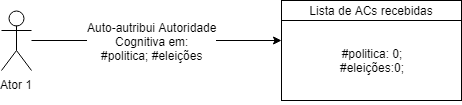
\includegraphics[scale=0.65]{4-proposta/diagrama_auto-autribuida.png}
\caption{Auto-atribuição de Autoridade Cognitiva.}
\label{fig:diagrama_auto-atribuida}
\end{figure}

Além de atribuir áreas de interesse uns aos outros, os atores podem utilizar \emph{tags} em formas de palavras-chave para atribuir uma descrição a um objeto na rede, como mostrado na figura \ref{fig:diagrama_palavras-chave}. As descrições propostas pelos atores podem auxiliar na identificação de áreas de interesse, auxiliando também na recuperação de informações por outros atores da rede (\cite{pereira_folkauthority:_2008}).

\begin{figure}[ht]
\centering
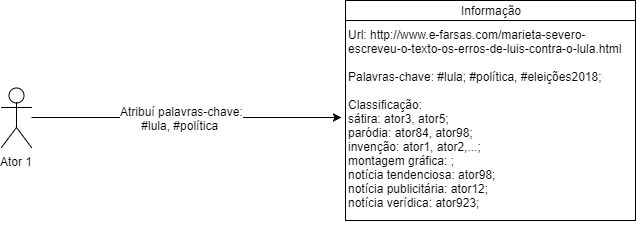
\includegraphics[scale=0.65]{4-proposta/diagrama_atribuicao_tags.png}
\caption{Atribuição de palavras-chave a uma informação.}
\label{fig:diagrama_palavras-chave}
\end{figure}

%----------------------------------------------------------------------------------------------------------------------------------------

\subsection{Autoridades Cognitivas possuem diferentes níveis}

Uma quantidade de AC pode ser possuída, seja ela pouca ou muita (\cite{Wilson1983}). Ou seja, iremos tratar AC como objetos que podem ser dados ou recebidos e uma quantidade destes pode ser possuída. Wilson ainda conclui que as pessoas, normalmente, expressam AC por meio de bases indiretas e que nem sempre é possível demonstrar essa autoridade em um valor ou escala mensurável. Portanto, propõe-se que existam duas listas: \textbf{lista de Autoridades Cognitivas recebidas}, que gerencia a AC que um indivíduo recebe de outro na rede; e uma \textbf{lista de Autoridades Cognitivas concedidas}, que gerencia as ACs que foram distribuídas para outro indivíduo na rede. Dessa forma é possível compilar um índice global que aumenta conforme outros usuários da rede reconhecem sua AC ( como ilustrado na figura \ref{fig:diagrama_relacionamento}). Esse índice pode ser analisado por outros atores e utilizado como indicador para saber se uma Autoridade Cognitiva é ou não reconhecida pelos seus pares. 

\begin{figure}[ht]
\centering
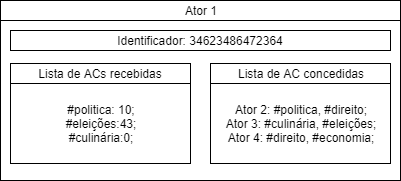
\includegraphics[scale=0.7]{4-proposta/diagrama_concebidos_recebidos.png}
\caption{Autoridades Cognitivas recebidas e concebidas.}
\label{fig:diagrama_recebidas_concebidas}
\end{figure}

Na figura \ref{fig:diagrama_recebidas_concebidas} percebe-se que na lista de ACs recebidas as áreas de interesse possuem valores destintos ilustrando o que acontece quando vários atores reconhecem a autoridade em uma mesma área. No assunto "eleições" o "Ator 1" foi reconhecido por 43 pessoas demonstrando um alto nível se comparado aos outros assuntos. Nota-se também que no assunto "culinária" o ator não foi reconhecido por ninguém, ilustrando um assunto que ele tem interesse porém ainda não é uma Autoridade Cognitiva para nenhum usuário na rede.



%----------------------------------------------------------------------------------------------------------------------------------------

\subsection{Autoridade Cognitiva envolve um relacionamento}

De acordo com \cite{Wilson1983} para a atribuição de AC é necessário o envolvimento entre no mínimo dois elementos. Além disso, \cite{pamela_j._mckenzie_justifying_2003} conclui que uma autoridade não é uma questão de inteligência ou especialidade, é uma questão de afinidade, confidência e admiração. Nota-se que não podemos considerar apenas como um relacionamento entre pessoas, pois é possível reconhecer autoridades em livros, instituições, instrumentos e organizações (\cite{soo_young_rieh_credibility_2010}). Ou seja, o ato de atribuir autoridade a alguma pessoa ou instituição é subjetiva e pessoal. O que pode ocasionar em erros por parte de quem reconhece uma autoridade, portanto é necessário uma checagem por parte de quem recebe, aceitando ou não ser AC sobre determinado assunto. Esse relacionamento é representado na figura \ref{fig:diagrama_relacionamento}.

\begin{figure}[ht]
\centering
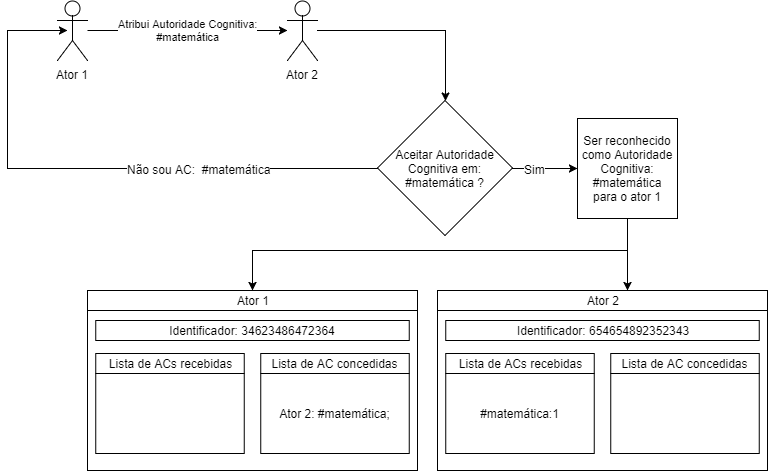
\includegraphics[scale=0.58]{4-proposta/diagrama_relacionamento.png}
\caption{Atribuição de Autoridade Cognitiva.}
\label{fig:diagrama_relacionamento}
\end{figure}

A figura \ref{fig:diagrama_relacionamento} demonstra ainda que AC é \textbf{unidirecional}: o fato de "A" ser uma autoridade para "B", não implica que "B" seja também uma autoridade para "A", mesmo que essa condição seja também possível (\cite{pereira_folkauthority:_2008}). Também é importante discutirmos sobre uma autoridade que foi renovada por outro ator, por exemplo, em uma situação onde "Ator 2" aceitou previamente a AC em matemática reconhecida por  um "Ator 0" ou atribuindo essa AC em si mesmo. Neste caso o "Ator 2" não precisará aceitar novamente, pois já possui reputação no assunto, mesmo que ela seja 0 (zero). 

\begin{figure}[ht]
\centering
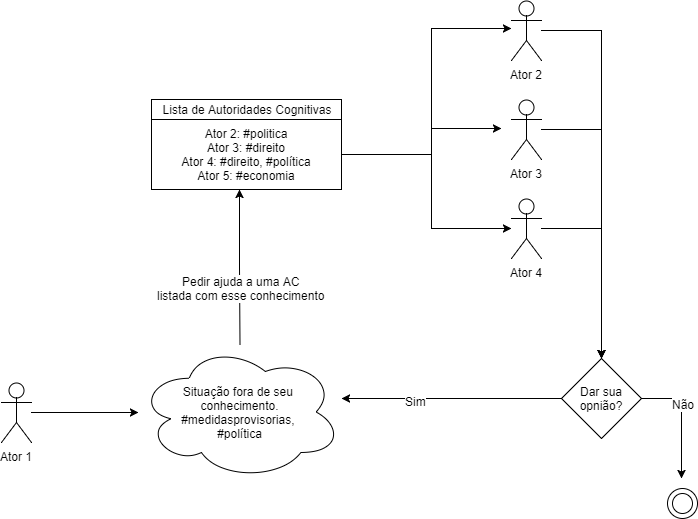
\includegraphics[scale=0.65]{4-proposta/diagrama_ajuda.png}
\caption{Solicitação de opinião para Autoridades Cognitivas.}
\label{fig:diagrama_ajuda}
\end{figure}

A partir do momento em que a relação de Autoridade Cognitiva é confirmada (proposta por quem reconhece e aceita por quem recebe), aquele que reconhece pode pedir ajuda para assuntos que são do interesse de quem aceitou a condição de AC. Uma AC não tem a obrigação de dar sua opinião sobre uma informação e pode ignorar a requisição. Esse relacionamento é ilustrado na figura \ref{fig:diagrama_ajuda}.

\begin{figure}[ht]
\centering
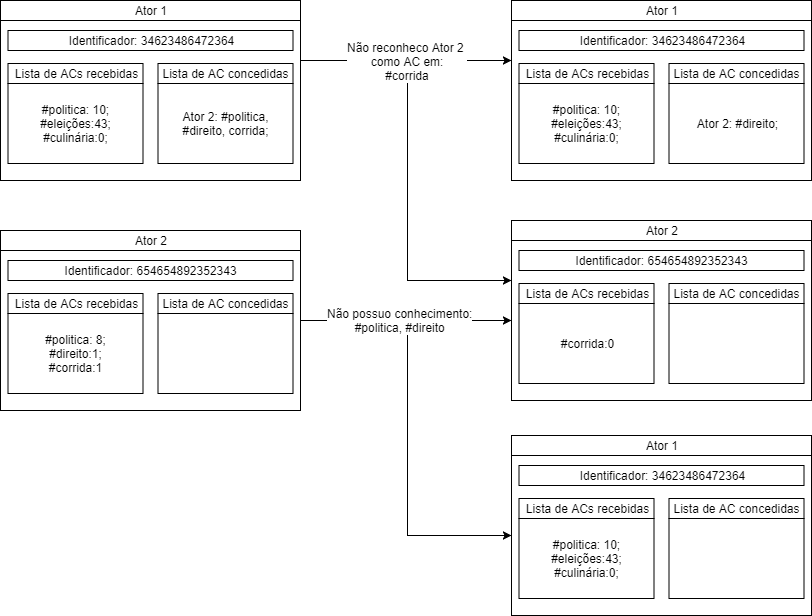
\includegraphics[scale=0.55]{4-proposta/diagrama_exclusao.png}
\caption{Exclusão de Autoridade Cognitiva.}
\label{fig:diagrama_exclusao}
\end{figure}

Um ator pode a qualquer momento reconsiderar uma AC atribuída por ele, assim como uma AC reconhecida pode renunciar uma Autoridade, como o ilustrado da figura \ref{fig:diagrama_exclusao}. O fato de um indivíduo "A" reconsiderar uma AC atribuída a um indivíduo "B", não significa que "B" não é mais uma AC, significa que o nível de AC de "B" diminuiu. Só é possível a eliminação total de um AC por parte do próprio indivíduo, pois uma Autoridade pode ser auto-atribuída. A figura \ref{fig:diagrama_exclusao} ainda mostra que mudança de de AC concebida ou recebida por parte de qualquer ator afeta os outros atores na rede.

%----------------------------------------------------------------------------------------------------------------------------------------

\subsection{Autoridades Cognitivas são diretamente relacionadas a credibilidade}

A influência de uma autoridade é aceitável pois esta é crível, digna de confiança (\cite{Wilson1983}). Portanto, além das diretrizes que permitem a identificação e organização das ACs devem existir mecanismos que permitam que os atores sinalizem confiança (ou desconfiança) nas informações compartilhadas na rede. 

O mecanismo proposto baseia-se na tipologia estudada por \cite{tandoc_defining_2017} que mapeia 6 formas de \emph{fake news}: (1) sátira; (2) paródia; (3) invenção; (4) montagem gráfica; (5) notícia publicitária; (6) notícia tendenciosa. Os atores devem ser capazes de classificar os objetos que trafegam na rede utilizando rótulos que representam os 6 tipos mapeados com a adição de mais um rótulo para expressar confiança: \textbf{notícia verídica}. A figura \ref{fig:diagrama_classificacao} representa esta ideia.

\begin{figure}[ht]
\centering
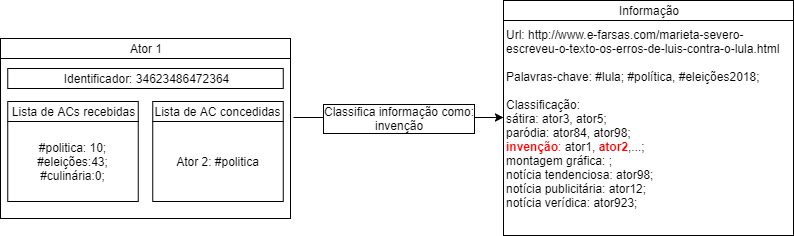
\includegraphics[scale=0.55]{4-proposta/diagrama_atribuicao_classificacao.png}
\caption{Classificação de um objeto na rede.}
\label{fig:diagrama_classificacao}
\end{figure}

Cada ator pode utilizar apenas uma classificação para cada objeto, sendo possível mudar posteriormente sua opinião. Essa regra busca evitar que alguns atores forcem uma classificação na rede.

Deve ser possível visualizar o índice completo da quantidade de atores que classificaram o objeto e qual classificação foi utilizada. Além disso priorizar a opinião dos atores considerados Autoridades Cognitivas no assunto em questão. Esse índice auxilia os outros atores da rede a identificar o objeto e decidirem por si mesmo qual a opinião deles sobre o mesmo.


%----------------------------------------------------------------------------------------------------------------------------------------

\section{Protótipo}

Este trabalho propõe o desenvolvimento de um sistema protótipo que implementará as diretrizes e fundamentos apresentados no modelo teórico, e funcionará como um identificador coletivo de notícias falsas. O protótipo proposto será composto por quatro elementos principais: três módulos e um banco de dados: \textbf{(1) interface gráfica}; \textbf{(2) processamento}; \textbf{(3) comunicação} e \textbf{(4) banco de dados}. Além destes, o sistema conta com a interação com uma API\footnote{Vem do termo Application Program Interface (Interface de Programação de Aplicação em Português), um conjunto de rotinas e padrões estabelecidos por um sistema para a utilização das suas funcionalidades para aplicativos externos ao sistema principal.} externa, que fornecerá os dados sobre contatos da rede social do usuário. Todas as partes devem se comunicar de acordo com o proposto na figura \ref{fig:arquitetura_sist_id_not_falsas}.

\begin{figure}[ht]
\centering
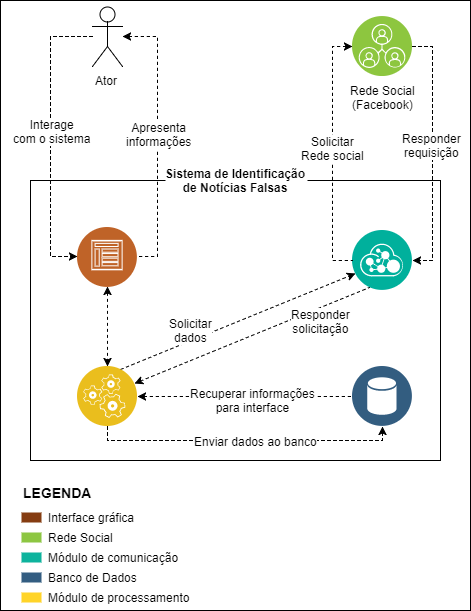
\includegraphics[scale=0.6]{4-proposta/arquitetura_do_sistema.png}
\caption{Arquitetura do sistema de identificação coletiva de notícias falsas.}
\label{fig:arquitetura_sist_id_not_falsas}
\end{figure}

\subsection{Interface gráfica}
Este elemento da arquitetura deve prover suporte ao usuário em termos de execução das operações dentro do sistema e de apresentação dos resultado das suas ações. As operações básicas planejadas de acordo com o modelo teórico são:

\begin{itemize}
    \item atribuir/remover autoridade cognitiva a um ator;
    \item inserir/buscar objeto (URL)
    \item organizar autoridade cognitiva recebida, incluindo aceitação/negação e auto-atribuição e remoção completa
    \item requisitar opinião de ator em relação a um objeto
    \item inserir/remover palavras-chave em um objeto
    \item inserir/remover classificação de um objeto
\end{itemize}

\subsection{Rede social}
Segundo \cite{nic.br_pesquisa_2017} o \emph{Facebook} e o \emph{Twitter} são as duas redes sociais mais populares no Brasil, neste trabalho optamos por focar no \emph{Facebook} pois além do grande público alcançado pela plataforma online, a empresa também detém o domínio de dois aplicativos de mensagens (\emph{Facebook Messenger e Whatsapp}), que de acordo com \cite{nic_newman_digital_2017} possuem um grande crescimento no Brasil. Portanto, neste trabalho utilizaremos a rede social do \emph{Facebook} para aplicar nosso modelo. Isso será possível graças a uma API (chamada \emph{The Graph API}) desenvolvida pela empresa. A \emph{Graph} proporciona formas de acesso ao gráfico social de usuários cadastrados (com devidas permissões) possibilitando recuperação de informações destes usuários, entre essas poderemos extrair a lista de amigos e informações públicas que caracterizam seus perfis online;
   
\subsection{Módulo de comunicação}
Este módulo recebe do solicitações do módulo de processamento, essas serão enviadas a um serviço externo. Neste trabalho esse módulo será o intermediário entre o protótipo e a rede social;
    
\subsection{Módulo de processamento}
É responsável pelo processamento das requisições realizadas pelo usuário na interface gráfica, por recuperar e inserir informações do banco de dados quando necessário, somar de autoridade cognitiva dos atores, somar o índice de classificação e palavras-chave dos objetos e requisitar ao módulo de comunicações informações das APIs externas; 
    
\subsection{Banco de dados}
É responsável pela persistência das informações e entidades que serão utilizados no sistema. Esse elemento é de grande importância, pois a modelagem das tabelas do banco de dados irão definir como iremos armazenar e recuperar as informações, tanto para a operação do sistema. A figura \ref{fig:mer} ilustra quais são as principais entidades existentes e como as tabelas do banco irão se relacionar. Observa-se que temos 4 entidades principais, com mais duas tabelas auxiliares totalizando 6 tabelas listadas, cada uma responsável pelo armazenamento de uma entidade no nosso sistema: 

    \begin{figure}[ht]
    \centering
    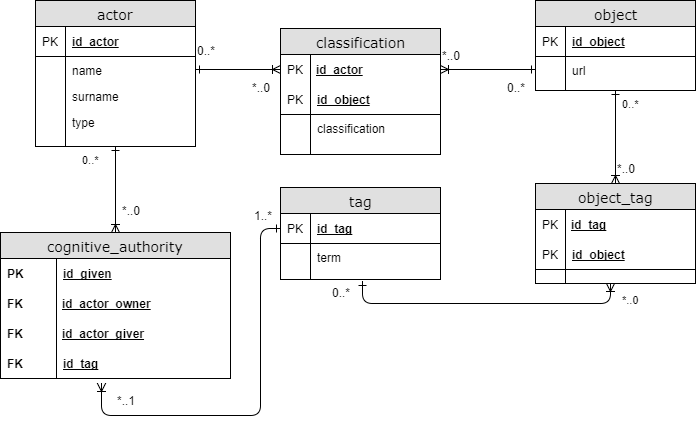
\includegraphics[scale=0.5]{4-proposta/mer.png}
    \caption{Modelo entidade relacionamento do banco de dados.}
    \label{fig:mer}
    \end{figure}

\begin{enumerate}
    \item \textbf{\emph{Actor} (Ator)}: representa os atores do sistema, possui os atributos \emph{id\_actor} (identificador único), \emph{name}(nome), \emph{surname} (sobrenome) e \emph{type}(tipo). O atributo \emph{type} é relativo ao tipo de ator, podendo representar, pessoa física, artista, instituição ou organização. Os outros atributos são auto-explicativos e foram idealizados apenas para propósito de identificação, porém outros atributos podem ser interessantes, como endereço, educação, entre outros. 
    
    Além dos atributos, a tabela \emph{actor} possui dois relacionamentos, um de zero para muitos com a tabela \emph{cognitive\_authority}, representando que cada entidade ator possui zero ou mais entidades de autoridades cognitivas concebidas e/ou recebidas. E um de muitos para muitos com a tabela \emph{object}, representando que um ator pode classificar zero ou mais objetos, que por sua vez, podem ser classificados por zero ou mais atores ;
    
    \item \textbf{\emph{Cognitve authority}}: esta tabela representa uma autoridade cognitiva recebida ou concedida, possui os seguintes atributos: 
    \begin{itemize}
        \item \emph{id\_received}: identificador único da tabela;
        \item \emph{id\_actor\_owner}: identificador de quem recebeu a autoridade cognitiva;
        \item \emph{id\_actor\_giver}: identificador do ator que concedeu a autoridade cognitiva; 
        \item \emph{id\_tag}: é o identificador único de uma \emph{tag} (rótulo); 
    \end{itemize}
    
    \item \textbf{\emph{Tag}}: é a entidade responsável pelos rótulos dos objetos e das AC no sistema cada \emph{tag} possui uma identificação única (\emph{id\_tag}, e um atributo queem uma cas armazenará o termo utilizado na rotulação (\emph{term}). Os relacionamentos presentes nesta tabela são com as tabelas  \emph{cognitive\_authority} e \emph{object\_tag}. A primeira é uma relação de um para muitos onde uma autoridade cognitiva dada ou recebida possui apenas um rótulo que a descreve. A segunda é uma relação muitos para muitos com a entidade \emph{object}, demonstrando que um rótulo pode estar presente em vários objetos distintos e um objeto pode conter vários rótulos distintos. Para possibilitar este relacionamento foi utilizado a entidade auxiliar \emph{object\_tag};
    
    \item \textbf{\emph{Object}}: esta entidade é responsável por armazenar dados sobre o objeto proposto no modelo, possui os seguintes atributos:
    \begin{itemize}
        \item \emph{id\_object}: é o identificador único do objeto;  
        \item \emph{url}: é a forma padronizada que foi escolhida para a representação da informação no sistema, este formato foi escolhido por sua ampla gama de usos, podendo representar documentos, sites, artigos, fotos, entre outros;
    \end{itemize}
    A tabela possui dois relacionamentos de muitos para muitos com as tabelas \emph{actor} e \emph{tag} , o primeiro  sinaliza que um ator pode classificar zero ou mais objetos que, podem ser classificados por zero ou mais atores. O segundo, mostra que um objeto possui zero ou mais rótulos que podem ser utilizados para descrever zero ou mais objetos. Essas relações se fazem possíveis pela utilização das tabelas auxiliares: \emph{obect\_tag} e \emph{classification}.
\end{enumerate}    

% --------------------------------------------------------------------------------------------------------------------

\section{Avaliação}

Pesquisas cientificas são realizadas visando o progresso ou aperfeiçoamento. Portanto, devem existir maneiras de quantificar esse progresso. De acordo com \cite{jayaratna_understanding_1994} nenhum processo, que visa a solução de um problema, pode ser considerado completo até que uma avaliação deste seja realizada. É esta avaliação que irá auxiliar na medição da efetividade da solução em frente ao problema encontrado. Se este elemento não for considerado, é impossível saber ao certo se o problema foi solucionado em algum nível.

\subsection{Abordagens de pesquisa}

Segundo \cite{chen_s._information_2011}, em pesquisas de avaliação podemos utilizar abordagens quantitativos, qualitativos e a mistura dos dois. \cite{creswell_research_2014} comenta que essas abordagens não são opostas, argumentado que um estudo pode ser mais qualitativo que quantitativo e vice-versa. Ele define as três abordagens da seguinte forma:

\begin{itemize}
    \item Pesquisa \textbf{qualitativa}: é um meio para explorar e entender o significado que os indivíduos ou grupos atribuem a um problema social ou humano. O processo de pesquisa envolve questões e procedimentos emergentes, os dados normalmente são coletados a partir da configuração de um participante. A análise de dados é construída de forma indutiva de temas particulares para gerais. E o pesquisador realiza suas interpretações do significado dos dados. O relatório final possui uma estrutura flexível. Aqueles que se envolvem nesta forma de inquérito apoiam um olhar um estilo indutivo de fazer pesquisa, com um foco no significado individual e na complexidade de uma situação (\cite{creswell_research_2014}).
    
    \item Pesquisa \textbf{quantitativa}: é um meio para testar teorias objetivas examinando a relação entre variáveis. Essas variáveis por sua vez, podem ser medidas, tipicamente com instrumentação, de modo que os dados possam ser analisados usando procedimentos estatísticos. O relatório escrito final possui uma estrutura definida que consiste em introdução, literatura e teoria, métodos, resultados e discussão. Aqueles que se envolvem nesta forma de investigação testam suas teorias de forma dedutiva, constroem proteções contra viés, controlam explicações alternativas e são capazes de generalizar e replicar suas descobertas (\cite{creswell_research_2014}).
    
    \item Pesquisa com \textbf{métodos mistos}: é uma abordagem de investigação que combina ou associa ambas as formas mostradas: qualitativas e quantitativas. Envolve pressupostos filosóficos, o uso de abordagens qualitativas e quantitativas e a mistura de ambas as abordagens em um estudo. Portanto, é mais do que simplesmente coletar e analisar ambos os tipos de dados, é o envolvimento de ambas as abordagens em conjunto, de modo que a força geral de um estudo seja maior do que a pesquisa qualitativa ou quantitativa (\cite{creswell_research_2014}).
\end{itemize}

Como forma de auxilio para a escolha da abordagem de pesquisa \cite{creswell_research_2014} apresenta um \emph{framework} relacionando três componentes: visões filosóficas do mundo; estratégias de investigação e métodos específicos. As quatro visões de mundo, segundo \cite{creswell_research_2014} são:

\subsection{Visões filosóficas}

\begin{enumerate}
    \item \textbf{Pós-positivismo}: Os pressupostos pós-positivistas representaram a forma tradicional de pesquisa, e essas são mais relacionadas a pesquisas quantitativas do que qualitativas. É chamado de pós-positivismo porque representa o pensamento após o positivismo, desafiando a noção tradicional da verdade absoluta do conhecimento e reconhecendo que não podemos ser "positivos" sobre nossas reivindicações de conhecimento ao estudar o comportamento e as ações dos seres humanos. Os problemas estudados pelos pós-positivistas refletem a necessidade de identificar e avaliar as causas que influenciam os resultados (\cite{creswell_research_2014});

    \item \textbf{Construtivismo}: Os construtivistas detêm pressupostos de que os indivíduos buscam a compreensão do mundo em que vivem e trabalham. Os indivíduos desenvolvem significados subjetivos de suas experiências. Essa perspectiva tem maior relação com uma abordagem qualitativa de pesquisa (\cite{creswell_research_2014});
    
    \item \textbf{Advocacia/Participativa}: Este grupo de pesquisadores detém os pressupostos filosóficos da abordagem advocacia / participação. Esta posição surgiu durante os anos de 1980 e 1990, fundamentada por indivíduos que sentiram que os pressupostos pós-positivistas impunham leis e teorias estruturais que não se encaixavam em indivíduos marginalizadas da nossa sociedade. Esta visão de mundo é normalmente vista com pesquisa qualitativa, mas pode ser utilizada como uma base para a pesquisa quantitativa (\cite{creswell_research_2014});
    
    \item \textbf{Pragmatismo}: O pragmatismo como visão de mundo surge de ações, situações e consequências, em vez de condições antecedentes (como no pós-positivismo). Existe uma preocupação com as aplicações, com o que funciona e as soluções para os problemas. Em vez de se concentrar em métodos, os pesquisadores enfatizam o problema da pesquisa e usam todas as abordagens disponíveis para entender o problema. Tem maior relação com os estudos de métodos mistos (\cite{creswell_research_2014}).
\end{enumerate}

Os principais elementos dessas visões de mundo podem ser observados na tabela \ref{tab:visoes_mundo}.

    \begin{center}
        \begin{table}[!htp]
            \caption{Diferentes visões de mundo e seus elementos}
            \label{tab:visoes_mundo}
            \begin{tabular}{|p{4.5cm}|p{10cm}|}
                \cline{1-2}                                 
                \hline
                {Pós-positivismo}                        &$\bullet$ Determinismo                             \\
                                                         &$\bullet$ Reducionismo                             \\
                                                         &$\bullet$ Observação empírica e medição            \\
                                                         &$\bullet$ Verificação de uma teoria                \\
                \hline
                {Construtivismo}                         &$\bullet$ Compreendimento                          \\
                                                         &$\bullet$ Múltiplos significados dos participantes \\
                                                         &$\bullet$ Construção social e histórica            \\
                                                         &$\bullet$ Geração de uma teoria                    \\
                \hline
                {Advocacia/Participativa}                &$\bullet$ Política                                 \\
                                                         &$\bullet$ Problema orientado a empoderamento       \\
                                                         &$\bullet$ Colaborativo                             \\
                                                         &$\bullet$ Orientado a mudança                      \\
                \hline
                {Pragmatismo}                            &$\bullet$ Consequência de ações                    \\
                                                         &$\bullet$ Centralizado em torno do problema        \\
                                                         &$\bullet$ Pluralismo                               \\
                                                         &$\bullet$ Orientado a práticas do mundo real       \\
                \hline
            \end{tabular}
        \end{table}
    \end{center}

\subsection{Estratégias de investigação}

Um pesquisador ainda deve ponderar sobre as estratégias de investigação que irá utilizar em sua pesquisa. Essas estratégias são designs ou modelos que fornecem uma direção específica para os procedimentos que serão realizados no design da pesquisa. \cite{creswell_research_2014} relaciona essas estratégias com suas abordagens de pesquisa, assim como ilustrado na tabela \ref{tab:estrategias_investigacao}.

    \begin{center}
        \begin{table}[!htp]
            \caption{Estratégias de investigação e abordagens de pesquisa}
            \label{tab:estrategias_investigacao}
            \begin{tabular}{|p{4.5cm}|p{5cm}|p{5cm}|}
                \hline
                Quantitativo                      & Qualitativo                     & Métodos mistos   \\
                \hline
                Designs Experimentais;              & Pesquisa de Narrativa;          & Sequencial; \\
                Designs não-experimentais, como entrevistas.     & Fenomenologia;       & Concorrente;    \\
                                                  & Etnografias;       & Transformativo.    \\
                                                  & Estudo de teorias fundamentadas;       &     \\
                                                  & Estudo de caso.       &     \\
                \hline
            \end{tabular}
        \end{table}
    \end{center}

\subsection{Métodos de pesquisa}

O terceiro elemento principal do \emph{framework} de \cite{creswell_research_2014} é o método de pesquisa, que envolve as formas de coleta, análise, e interpretação dos dados que os pesquisadores propõem nos seus estudos. A tabela \ref{tab:metodos_pesquisa} ilustra os métodos de pesquisa discutidos por \cite{creswell_research_2014}.

    \begin{center}
        \begin{table}[!htp]
            \caption{Métodos e abordagens de pesquisa}
            \label{tab:metodos_pesquisa}
            \begin{tabular}{|p{4.5cm}|p{5cm}|p{5cm}|}
                \hline
                Quantitativo                      & Qualitativo                     & Métodos mistos   \\
                \hline
                Pré-determinados              & Métodos emergentes          & Ambos \\
                \hline
                Questões baseadas fechadas com respostas diretas & Questões abertas       & Ambos    \\
                \hline
                Dados de performance, atitude, de observação e de censo  & Dados de entrevistas, de observação, de documentos e áudio-visual       &  Todas as possibilidades    \\
                \hline
                Análise estatística & Análise textual e de imagens       &  Ambas   \\
                \hline
                Interpretação estatística  & Interpretação de temas e padrões       & Ambas    \\
                \hline
            \end{tabular}
        \end{table}
    \end{center}

\subsection{Estratégia de pesquisa proposta}

Baseado nas características apresentadas no estudo de \cite{creswell_research_2014}, foi identificado que este estudo utilizará uma abordagem quantitativa de pesquisa e portanto se utilizará dos métodos quantitativos citados. Portanto, foi escolhido o seguinte cenário:

\begin{itemize}
    \item Visão filosófica: Pós-positiva ;
    \item Estratégia de investigação: Entrevistas e experimentos;
    \item Métodos de pesquisa: Entrevistas com questões fechadas, experimentos com cenários pré-determinados, e extração de dados numéricos;
    \item É responsabilidade do pesquisador: Testar a teoria, identificar de variáveis de estudo, relacionar de variáveis em questões e hipóteses, utilizar padrões de validade e confiabilidade, observar e avaliar informações numericamente, utilizar uma abordagem imparcial, empregar procedimentos estatísticos.
\end{itemize}		% proposta
%\chapter{Metodologia}

Aqui vou colocar como será desenvolvido o prototipo?

módulos tipo bd, api, ui? ou preciso adicionar documento de requisito diagramas de classes, definir linguagem, paradigma etc?	% experimentação e validação
\chapter{Cronograma}

  O cronograma apresentado, considera uma solicitação de extensão do prazo para a defesa final. Sem essa extensão o prazo final é de Julho de 2018. As atividades necessárias para a execução do trabalho são descritas a seguir:
	
\begin{enumerate}	
	\item Desenvolvimento de casos de uso: desenvolver os casos de uso utilizando o modelo conceitual; \label{atividade1}
	
	\item Desenvolvimento o protótipo: Construção do protótipo proposto, considerando sua arquitetura e modelo de banco de dados. Esta atividade envolve testes e manutenção; \label{atividade2}
	
	\item Escrita da dissertação: Catalogar e escrever os resultados parciais e finais, e compilá-los em um formato de dissertação; \label{atividade3}
	
	\item Compilação dos experimentos: Identificar variáveis de estudo e relacioná-las com a hipótese proposta para o desenvolvimento dos experimentos; \label{atividade4}
	
	\item Execução experimentos: Realizar experimentação com usuários reais. Empregar métodos estatísticos para análise dos dados obtidos com os experimentos; \label{atividade5}
	
	\item Escrita de artigo: compilação dos resultados obtidos em formato de artigo. \label{atividade6}
	
	\item Apresentação da pesquisa: Apresentação da solução desenvolvida para a Banca. \label{atividade7}
	
\end{enumerate}

A Tabela \ref{tabela:cronograma} apresenta o cronograma de execução do trabalho.

\begin{table}[ht]
\small
\centering

\begin{tabular}{|l|c|c|c|c|c|c|c|c|c|c|}
\hline & \multicolumn{10}{|c|}{\textbf{Período}} \\ \cline{2-11}
\textbf{Atividades}                     &Fev     &Mar      &Abr     &Mai     &Jun      &Jul      &Ago      &Set     &Out     &Nov      
\\ \hline

\ref{atividade1} Desenvolvimento de casos de uso  &$\bullet$& &        &         &         &         &     &        &       &     
\\ \hline

\ref{atividade2} Desenvolvimento do protótipo    &$\bullet$ &$\bullet$&$\bullet$&$\bullet$&$\bullet$&$\bullet$&       &       &      &
\\ \hline

\ref{atividade3} Escrita da dissertação                &         &$\bullet$ &$\bullet$ &$\bullet$&$\bullet$&$\bullet$&$\bullet$&$\bullet$&$\bullet$&
\\ \hline

\ref{atividade4} Compilação dos experimentos    &         &         &$\bullet$&$\bullet$&     &      &     &   &   &
\\ \hline

\ref{atividade5} Execução de experimentos               &      &      &      &       &$\bullet$&$\bullet$&$\bullet$&$\bullet$&$\bullet$&
\\ \hline

\ref{atividade6} Escrita de artigo             &     &$\bullet$ &$\bullet$&$\bullet$&$\bullet$&$\bullet$&$\bullet$&$\bullet$&$\bullet$&$\bullet$
\\ \hline

\ref{atividade7} Apresentação da pesquisa &         &         &         &         &         &         &    &    &     &$\bullet$
\\ \hline

\end{tabular}

\caption{Cronograma das Atividades}\label{tabela:cronograma}
\end{table}

%\chapter{Conclusão}

Realmente preciso de ajuda aqui...
To querendo juntar a revisao sistematica e a viabilidade e colocar tudo aqui, mostrando que o tema e hot topic etc   % conclusão

%=====================================================

% Estilos de bibliografia recomendados (só descomentar um estilo!)
%\bibliographystyle{apalike-ptbr}	% [Maziero et al., 2006]
%\bibliographystyle{plain}		% [1], [1, 2]
%\bibliographystyle{alpha}		% [Maz06], ...
\bibliographystyle{plainnat}		% vide Google "LaTeX Natbib"

% base de bibliografia (BibTeX)
\bibliography{referencias1}
%\bibliography{file1, file2, file3} % se tiver mais de um arquivo BibTeX

%=====================================================

% inclusão de apêndices
%\appendix
%\chapter{Exemplo de anexo}

%=====================================================

Os apêndices são uma extensão do texto, destacados deste para evitar descontinuidade na sequência lógica ou alongamento excessivo de determinado assunto ou tópico secundário dentro dos capítulos da dissertação ou da tese. São contribuições que servem para esclarecer, complementar, provar ou confirmar as ideias apresentadas no texto dos capítulos e que são importantes para a compreensão dos mesmos.

Todos os apêndices devem vir após as referências bibliográficas e devem ser enumerados por letras maiúsculas (A, B, C, ...).

%=====================================================

\section{Uma Seção}

\lipsum[20-23]

%=====================================================

\subsection{Uma Subseção}

\lipsum[30-33]

%=====================================================

\subsection{Outra Subseção}

Exemplo de lista simples com dois níveis: Exemplo de lista simples com dois níveis: Exemplo de lista simples com dois níveis: Exemplo de lista simples com dois níveis: Exemplo de lista simples com dois níveis: Exemplo de lista simples com dois níveis: Exemplo de lista simples com dois níveis: Exemplo de lista simples com dois níveis: Exemplo de lista simples com dois níveis.

\begin{itemize}

\item Banana, Banana, Banana, Banana, Banana, Banana, Banana, Banana, Banana, Banana, Banana, Banana, Banana, Banana, Banana, Banana, Banana, Banana, Banana, Banana, Banana, Banana, Banana, Banana.

\begin{itemize}

\item Caturra, Caturra, Caturra, Caturra, Caturra, Caturra, Caturra, Caturra, Caturra, Caturra, Caturra, Caturra, Caturra, Caturra, Caturra, Caturra, Caturra, Caturra, Caturra.

\item da Terra, da Terra, da Terra, da Terra, da Terra, da Terra, da Terra, da Terra, da Terra, da Terra, da Terra, da Terra, da Terra, da Terra, da Terra, da Terra, da Terra, da Terra.

\end{itemize}

\item Laranja, Laranja, Laranja, Laranja, Laranja, Laranja, Laranja, Laranja, Laranja, Laranja, Laranja, Laranja, Laranja, Laranja, Laranja, Laranja.

\begin{itemize}

\item Bahia, Bahia, Bahia, Bahia, Bahia, Bahia, Bahia, Bahia, Bahia, Bahia, Bahia, Bahia, Bahia, Bahia, Bahia, Bahia, Bahia, Bahia.

\item Lima, Lima, Lima, Lima, Lima, Lima, Lima, Lima, Lima, Lima, Lima, Lima, Lima, Lima, Lima, Lima, Lima, Lima, Lima, Lima, Lima, Lima, Lima, Lima, Lima, Lima, Lima, Lima, Lima.

\end{itemize}

\end{itemize}

Exemplo de lista numerada com dois níveis: Exemplo de lista numerada com dois níveis: Exemplo de lista numerada com dois níveis: Exemplo de lista numerada com dois níveis: Exemplo de lista numerada com dois níveis: Exemplo de lista numerada com dois níveis: Exemplo de lista numerada com dois níveis: Exemplo de lista numerada com dois níveis.

\begin{enumerate}

\item Banana, Banana, Banana, Banana, Banana, Banana, Banana, Banana, Banana, Banana, Banana, Banana, Banana, Banana, Banana, Banana, Banana, Banana, Banana, Banana, Banana, Banana, Banana, Banana.

\begin{enumerate}

\item Caturra, Caturra, Caturra, Caturra, Caturra, Caturra, Caturra, Caturra, Caturra, Caturra, Caturra, Caturra, Caturra, Caturra, Caturra, Caturra, Caturra, Caturra, Caturra.

\item da Terra, da Terra, da Terra, da Terra, da Terra, da Terra, da Terra, da Terra, da Terra, da Terra, da Terra, da Terra, da Terra, da Terra, da Terra, da Terra, da Terra, da Terra.

\end{enumerate}

\item Laranja, Laranja, Laranja, Laranja, Laranja, Laranja, Laranja, Laranja, Laranja, Laranja, Laranja, Laranja, Laranja, Laranja, Laranja, Laranja.

\begin{enumerate}

\item Bahia, Bahia, Bahia, Bahia, Bahia, Bahia, Bahia, Bahia, Bahia, Bahia, Bahia, Bahia, Bahia, Bahia, Bahia, Bahia, Bahia, Bahia.

\item Lima, Lima, Lima, Lima, Lima, Lima, Lima, Lima, Lima, Lima, Lima, Lima, Lima, Lima, Lima, Lima, Lima, Lima, Lima, Lima, Lima, Lima, Lima, Lima, Lima, Lima, Lima, Lima, Lima.

\end{enumerate}

\end{enumerate}

Exemplo de lista descritiva com dois níveis: Exemplo de lista descritiva com dois níveis: Exemplo de lista descritiva com dois níveis: Exemplo de lista descritiva com dois níveis: Exemplo de lista descritiva com dois níveis: Exemplo de lista descritiva com dois níveis: Exemplo de lista descritiva com dois níveis: Exemplo de lista descritiva com dois níveis: Exemplo de lista descritiva com dois níveis.

\begin{description}

\item [Banana]: Banana, Banana, Banana, Banana, Banana, Banana, Banana, Banana, Banana, Banana, Banana, Banana, Banana, Banana, Banana, Banana, Banana, Banana, Banana, Banana, Banana, Banana, Banana.

\begin{description}

\item [Caturra]: Caturra, Caturra, Caturra, Caturra, Caturra, Caturra, Caturra, Caturra, Caturra, Caturra, Caturra, Caturra, Caturra, Caturra, Caturra, Caturra, Caturra, Caturra.

\item [da Terra]: da Terra, da Terra, da Terra, da Terra, da Terra, da Terra, da Terra, da Terra, da Terra, da Terra, da Terra, da Terra, da Terra, da Terra, da Terra, da Terra, da Terra.

\end{description}

\item [Laranja]: Laranja, Laranja, Laranja, Laranja, Laranja, Laranja, Laranja, Laranja, Laranja, Laranja, Laranja, Laranja, Laranja, Laranja, Laranja.

\begin{description}

\item [Bahia]: Bahia, Bahia, Bahia, Bahia, Bahia, Bahia, Bahia, Bahia, Bahia, Bahia, Bahia, Bahia, Bahia, Bahia, Bahia, Bahia, Bahia.

\item [Lima]: Lima, Lima, Lima, Lima, Lima, Lima, Lima, Lima, Lima, Lima, Lima, Lima, Lima, Lima, Lima, Lima, Lima, Lima, Lima, Lima, Lima, Lima, Lima, Lima, Lima, Lima, Lima, Lima.

\end{description}

\end{description}

%=====================================================


\end{document}

%=====================================================
